\documentclass[11pt,a4paper]{article}

\usepackage[T1]{fontenc}
\usepackage[utf8]{inputenc}
\usepackage{textcomp}
\DeclareUnicodeCharacter{2212}{\ensuremath{-}}
\DeclareUnicodeCharacter{00B0}{\ensuremath{^\circ}}
\usepackage{lmodern}
\usepackage[margin=2.3cm]{geometry}
\usepackage{amsmath,amssymb}
\usepackage{graphicx}
\usepackage{booktabs}
\usepackage{siunitx}
\usepackage{xcolor}
\usepackage[font=small,labelfont=bf]{caption}
\usepackage{microtype}
\usepackage[section]{placeins}
\usepackage[colorlinks=true,linkcolor=blue!50!black,citecolor=blue!50!black,urlcolor=blue!50!black]{hyperref}

\sisetup{detect-all, per-mode=symbol}
\graphicspath{{figures/}}
\newcommand{\nangleCeiling}{45}
\newcommand{\nangleFloor}{-35}
\newcommand{\nangleLeft}{-59}
\newcommand{\nangleListenerwall}{-5}
\newcommand{\nangleRight}{46}
\newcommand{\nangleSpeakerwall}{151}
\newcommand{\ncolDomeFirFit}{1.58}
\newcommand{\ncolDomeFirPir}{1.35}
\newcommand{\ncolDomeFirRefl}{1.70}
\newcommand{\ncolDomeFirSteady}{1.62}
\newcommand{\ncolDomeFirVert}{1.86}
\newcommand{\ncolDomeFirVertDip}{10.4}
\newcommand{\ncolDomeLrEightFit}{2.02}
\newcommand{\ncolDomeLrEightPir}{1.65}
\newcommand{\ncolDomeLrEightRefl}{2.44}
\newcommand{\ncolDomeLrEightSteady}{2.13}
\newcommand{\ncolDomeLrEightVert}{3.67}
\newcommand{\ncolDomeLrEightVertDip}{11.7}
\newcommand{\ncolDomeLrFourFit}{2.11}
\newcommand{\ncolDomeLrFourPir}{1.73}
\newcommand{\ncolDomeLrFourRefl}{2.75}
\newcommand{\ncolDomeLrFourSteady}{2.25}
\newcommand{\ncolDomeLrFourVert}{4.58}
\newcommand{\ncolDomeLrFourVertDip}{12.7}
\newcommand{\ncolDomeLrTwoFit}{2.20}
\newcommand{\ncolDomeLrTwoMoreFit}{4}
\newcommand{\ncolDomeLrTwoMorePir}{8}
\newcommand{\ncolDomeLrTwoMoreRefl}{14}
\newcommand{\ncolDomeLrTwoMoreSteady}{7}
\newcommand{\ncolDomeLrTwoMoreVert}{20}
\newcommand{\ncolDomeLrTwoPir}{1.87}
\newcommand{\ncolDomeLrTwoRefl}{3.13}
\newcommand{\ncolDomeLrTwoSteady}{2.41}
\newcommand{\ncolDomeLrTwoVert}{5.51}
\newcommand{\ncolDomeLrTwoVertDip}{15.2}
\newcommand{\ncolDomeRedFit}{25}
\newcommand{\ncolDomeRedPir}{22}
\newcommand{\ncolDomeRedRefl}{38}
\newcommand{\ncolDomeRedSteady}{28}
\newcommand{\ncolDomeRedVert}{59}
\newcommand{\ncolDomeRedVertDip}{18}
\newcommand{\ncolWgFirFit}{0.76}
\newcommand{\ncolWgFirPir}{0.64}
\newcommand{\ncolWgFirRefl}{0.99}
\newcommand{\ncolWgFirSteady}{0.83}
\newcommand{\ncolWgFirVert}{1.58}
\newcommand{\ncolWgFirVertDip}{11.7}
\newcommand{\ncolWgLrEightFit}{1.34}
\newcommand{\ncolWgLrEightPir}{1.04}
\newcommand{\ncolWgLrEightRefl}{1.81}
\newcommand{\ncolWgLrEightSteady}{1.45}
\newcommand{\ncolWgLrEightVert}{3.35}
\newcommand{\ncolWgLrEightVertDip}{10.9}
\newcommand{\ncolWgLrFourFit}{1.50}
\newcommand{\ncolWgLrFourPir}{1.19}
\newcommand{\ncolWgLrFourRefl}{2.11}
\newcommand{\ncolWgLrFourSteady}{1.65}
\newcommand{\ncolWgLrFourVert}{3.99}
\newcommand{\ncolWgLrFourVertDip}{10.7}
\newcommand{\ncolWgLrTwoFit}{1.63}
\newcommand{\ncolWgLrTwoMoreFit}{8}
\newcommand{\ncolWgLrTwoMorePir}{15}
\newcommand{\ncolWgLrTwoMoreRefl}{12}
\newcommand{\ncolWgLrTwoMoreSteady}{9}
\newcommand{\ncolWgLrTwoMoreVert}{14}
\newcommand{\ncolWgLrTwoPir}{1.37}
\newcommand{\ncolWgLrTwoRefl}{2.37}
\newcommand{\ncolWgLrTwoSteady}{1.80}
\newcommand{\ncolWgLrTwoVert}{4.54}
\newcommand{\ncolWgLrTwoVertDip}{11.3}
\newcommand{\ncolWgRedFit}{49}
\newcommand{\ncolWgRedPir}{47}
\newcommand{\ncolWgRedRefl}{53}
\newcommand{\ncolWgRedSteady}{50}
\newcommand{\ncolWgRedVert}{60}
\newcommand{\ncolWgRedVertDip}{-9}
\newcommand{\ncurveDomeFirEarly}{0.69}
\newcommand{\ncurveDomeFirFit}{1.29}
\newcommand{\ncurveDomeFirPir}{1.04}
\newcommand{\ncurveDomeFirPirDip}{2.02}
\newcommand{\ncurveDomeFirRoom}{1.32}
\newcommand{\ncurveDomeFirRoomDip}{3.01}
\newcommand{\ncurveDomeLrEightEarly}{0.78}
\newcommand{\ncurveDomeLrEightFit}{1.39}
\newcommand{\ncurveDomeLrEightPir}{1.09}
\newcommand{\ncurveDomeLrEightPirDip}{1.81}
\newcommand{\ncurveDomeLrEightRoom}{1.48}
\newcommand{\ncurveDomeLrEightRoomDip}{2.72}
\newcommand{\ncurveDomeLrFourEarly}{0.70}
\newcommand{\ncurveDomeLrFourFit}{1.24}
\newcommand{\ncurveDomeLrFourPir}{0.96}
\newcommand{\ncurveDomeLrFourPirDip}{1.56}
\newcommand{\ncurveDomeLrFourRoom}{1.36}
\newcommand{\ncurveDomeLrFourRoomDip}{2.37}
\newcommand{\ncurveDomeLrTwoEarly}{0.59}
\newcommand{\ncurveDomeLrTwoFit}{0.97}
\newcommand{\ncurveDomeLrTwoPir}{0.77}
\newcommand{\ncurveDomeLrTwoPirDip}{1.21}
\newcommand{\ncurveDomeLrTwoRoom}{1.11}
\newcommand{\ncurveDomeLrTwoRoomDip}{1.88}
\newcommand{\ncurveWgFirEarly}{0.24}
\newcommand{\ncurveWgFirFit}{0.43}
\newcommand{\ncurveWgFirPir}{0.35}
\newcommand{\ncurveWgFirPirDip}{1.75}
\newcommand{\ncurveWgFirRoom}{0.48}
\newcommand{\ncurveWgFirRoomDip}{2.49}
\newcommand{\ncurveWgLrEightEarly}{0.44}
\newcommand{\ncurveWgLrEightFit}{0.83}
\newcommand{\ncurveWgLrEightPir}{0.63}
\newcommand{\ncurveWgLrEightPirDip}{1.51}
\newcommand{\ncurveWgLrEightRoom}{0.92}
\newcommand{\ncurveWgLrEightRoomDip}{2.18}
\newcommand{\ncurveWgLrFourEarly}{0.45}
\newcommand{\ncurveWgLrFourFit}{0.85}
\newcommand{\ncurveWgLrFourPir}{0.64}
\newcommand{\ncurveWgLrFourPirDip}{1.24}
\newcommand{\ncurveWgLrFourRoom}{0.95}
\newcommand{\ncurveWgLrFourRoomDip}{1.84}
\newcommand{\ncurveWgLrTwoEarly}{0.37}
\newcommand{\ncurveWgLrTwoFit}{0.68}
\newcommand{\ncurveWgLrTwoPir}{0.51}
\newcommand{\ncurveWgLrTwoPirDip}{0.84}
\newcommand{\ncurveWgLrTwoRoom}{0.81}
\newcommand{\ncurveWgLrTwoRoomDip}{1.35}
\newcommand{\ndelayCeiling}{3.6}
\newcommand{\ndelayFloor}{1.9}
\newcommand{\ndelayLeft}{3.5}
\newcommand{\ndelayListenerwall}{13.4}
\newcommand{\ndelayRight}{9.0}
\newcommand{\ndelaySpeakerwall}{4.4}
\newcommand{\ndirectShare}{6.6}
\newcommand{\nearlyDirect}{36}
\newcommand{\nearlyVert}{27}
\newcommand{\nfirstShare}{11}
\newcommand{\nlateShare}{82}
\newcommand{\nnotchDomeFirCeilingDepth}{8}
\newcommand{\nnotchDomeFirCeilingWidth}{32}
\newcommand{\nnotchDomeFirFloorDepth}{21}
\newcommand{\nnotchDomeFirFloorWidth}{48}
\newcommand{\nnotchDomeLrFourCeilingDepth}{10}
\newcommand{\nnotchDomeLrFourCeilingWidth}{387}
\newcommand{\nnotchDomeLrFourFloorDepth}{41}
\newcommand{\nnotchDomeLrFourFloorWidth}{611}
\newcommand{\nnotchDomeLrTwoCeilingDepth}{13}
\newcommand{\nnotchDomeLrTwoCeilingWidth}{465}
\newcommand{\nnotchDomeLrTwoFloorDepth}{27}
\newcommand{\nnotchDomeLrTwoFloorWidth}{745}
\newcommand{\nnotchWgFirCeilingDepth}{9}
\newcommand{\nnotchWgFirCeilingWidth}{32}
\newcommand{\nnotchWgFirFloorDepth}{28}
\newcommand{\nnotchWgFirFloorWidth}{64}
\newcommand{\nnotchWgLrFourCeilingDepth}{8}
\newcommand{\nnotchWgLrFourCeilingWidth}{344}
\newcommand{\nnotchWgLrFourFloorDepth}{27}
\newcommand{\nnotchWgLrFourFloorWidth}{633}
\newcommand{\nnotchWgLrTwoCeilingDepth}{9}
\newcommand{\nnotchWgLrTwoCeilingWidth}{410}
\newcommand{\nnotchWgLrTwoFloorDepth}{23}
\newcommand{\nnotchWgLrTwoFloorWidth}{778}
\newcommand{\npirBiasLow}{0.8}
\newcommand{\npirBiasMax}{2.6}
\newcommand{\nrtHi}{0.68}
\newcommand{\nrtLo}{0.26}
\newcommand{\nrtMedian}{0.40}
\newcommand{\nsideShare}{31}
\newcommand{\nspBiasFir}{0.4}
\newcommand{\nspBiasLrEight}{1.7}
\newcommand{\nspBiasLrFour}{1.8}
\newcommand{\nspBiasLrTwo}{1.8}
\newcommand{\ntreated}{72}
\newcommand{\nvertHi}{52}
\newcommand{\nvertLo}{33}
\newcommand{\nvertShare}{41}
\newcommand{\nvertTreated}{50}
\newcommand{\nvertUntreated}{39}
\newcommand{\nwEr}{0.01}
\newcommand{\nwErEarly}{0.53}
\newcommand{\nwErTwo}{0.02}
\newcommand{\nwLw}{0.11}
\newcommand{\nwLwEarly}{0.40}
\newcommand{\nwLwTwo}{0.08}
\newcommand{\nwSp}{0.89}
\newcommand{\nwSpEarly}{0.07}
\newcommand{\nwSpTwo}{0.90}

\makeatletter
\newcommand{\rows}[1]{\@@input tables/#1.tex }
\makeatother

\newcommand{\vect}[1]{\mathbf{#1}}
\newcommand{\dd}{\,\mathrm{d}}
\newcommand{\jj}{\mathrm{j}}

\title{CTA-2034 in Simulated Rooms:\\What the Listener Receives, Direction by Direction\\[4pt]
\large The spinorama's weights against 300 domestic listening rooms,\\and a two-way loudspeaker with
Linkwitz-Riley and brickwall crossovers}
\author{}
\date{Technical report --- simulation code and data:\\
\url{https://github.com/Arnwald/cta2034-room-study}}

\begin{document}
\maketitle

\begin{abstract}
The curves of ANSI/CTA-2034-A (Listening Window, Early Reflections, Sound Power and the Predicted
In-Room Response, PIR) are weighted means of the power a loudspeaker radiates in 70 directions on
two orbits. The energy reaching a listener in a room is also a weighted mean of the power radiated
in every direction, with weights set by the paths' lengths and absorptions. We compute those weights
in 300 simulated domestic rooms (specular images up to the third order and a diffuse field fed
direction by direction; reverberation time \nrtMedian\,s at 1\,kHz, median) and compare them with
the standard's, using a two-way bookshelf loudspeaker whose far field is known over the whole
sphere, with a plain dome tweeter or a tweeter in a waveguide matched to the woofer at the
crossover, and LR2, LR4, LR8 or brickwall FIR crossovers. Three hypotheses were tested: that the
standard under-weighs the vertical directions, that the Listening Window hides the lobing of
low-slope crossovers, and that a weighting faithful to the received energy would show a brickwall
crossover removing most of the off-axis colouration. The floor and ceiling bring \nvertShare\,\% of
the first reflections' energy (\nvertTreated\,\% where the side walls are treated), the share the
Early Reflections give them, and their reflections leave the loudspeaker at angles the standard
brackets; the Listening Window's asymmetry matches where listeners sit. The weights themselves are
off: the first reflections carry \nfirstShare\,\% of the steady-state energy, against 44\,\% in the PIR,
and the rooms are predicted to within their own spread by about $\nwLw\,\mathrm{LW} +
\nwSp\,\mathrm{SP}$, where the PIR is 1.7 to 2.1\,dB RMS off; the two-orbit sound power shows about half
of the power lost to lobing. Averaging over directions, in the standard's curves as in the room, fills
the notches the crossover digs into each reflection: the floor and ceiling bounces of an LR4 two-way
carry notches of 10 to 40\,dB a third of an octave wide, which the averages reduce to a 2\,dB dip, and
the averages rank LR2 as the smoothest Linkwitz-Riley crossover while its reflections are the most
coloured. Read path by path, a brickwall crossover removes about 60\,\% of the colouration of the floor
and ceiling bounces (\ncolDomeRedVert\,\% with the plain dome, \ncolWgRedVert\,\% with the waveguide),
leaving notches as deep but ten to thirteen times narrower; the in-room curve becomes smoother only when the
drivers' directivities match at the crossover. Added with their phases at the listener's ears and
smoothed by the auditory filters, the paths change the steady state little; in the early sound at a
fixed point the comb of the floor and ceiling bounces outweighs any crossover's colouration, and the
Linkwitz-Riley notch, which takes these reflections out near the crossover, removes their comb there.
\end{abstract}

\tableofcontents

% =============================================================================================
\section{Introduction}

ANSI/CTA-2034-A \cite{cta2034a} describes a loudspeaker by 70 far-field measurements: a horizontal and
a vertical orbit around a reference axis, every $10^\circ$. Its curves average them: the
\emph{Listening Window} (LW) over the directions toward a group of listeners, the \emph{Early
Reflections} (ER) over the directions of the first reflections in a typical room, the \emph{Sound
Power} (SP) over all 70 directions, each weighted by the solid angle it stands for. Their mix, the
\emph{Predicted In-Room Response}
\begin{equation}
\mathrm{PIR} = 0.12\,\mathrm{LW} + 0.44\,\mathrm{ER} + 0.44\,\mathrm{SP},
\end{equation}
estimates the steady-state response measured at the listening position. The curves and the
prediction come from Devantier's work at Harman \cite{devantier2002}, the reflection directions from
a survey of domestic listening rooms; they are central to the work of Toole and Olive on loudspeaker
preference \cite{toole2018,olive2004}.

The standard was written for the measurement systems of its time, two orbits on a turntable, and
much of its practice grew around passive loudspeakers. Three objections motivated this study:

\begin{enumerate}
\item The vertical directions weigh less than the horizontal ones (two of the nine directions of the
Listening Window, two of the five bounces of the Early Reflections), while domestic rooms are wider
than high, and floors and ceilings are harder to treat than walls.
\item The Listening Window, $\pm30^\circ$ horizontally but $\pm10^\circ$ vertically, would hide the
vertical lobing of the low-slope crossovers of passive loudspeakers.
\item A weighting closer to the energy actually received would reveal that a brickwall crossover,
which leaves the drivers overlapping over a narrow band, removes most of the off-axis colouration of
a Linkwitz-Riley crossover \cite{demion2026}.
\end{enumerate}

Each of the standard's curves is a weighted mean of the power responses in the 70 directions. A room
does the same: in steady state, and once the paths are added in power (which a spatial average over
a few tenths of a metre achieves above the room's transition frequency), the energy at the listener
is a sum over paths of the power the loudspeaker radiates in each path's direction times the path's
weight. The comparison is thus between two sets of weights over directions. We compute the rooms'
in 300 simulated domestic listening rooms (section~\ref{sec:rooms}), with a loudspeaker whose far
field is known over the whole sphere (section~\ref{sec:loudspeaker}), and compare them with the
standard's (section~\ref{sec:standard}): where the energy leaves the loudspeaker, how much of it each
kind of path carries, how well the PIR predicts the rooms, and what an updated weighting gives. The
loudspeaker then comes with four crossovers, to test the third objection
(section~\ref{sec:crossovers}).

The curves follow CTA-2034-A as it is commonly implemented, the Early Reflections being the mean of
its five bounces. CTA-2034-B was published in July 2024 \cite{cta2034b}; its changes were not checked.

% =============================================================================================
\section{The standard's curves as weights over directions}
\label{sec:cta}

The two orbits pass through the reference axis. In the loudspeaker's frame ($x$ to the right as seen
from the listener, $y$ up, $z$ forward), the horizontal orbit at angle $h$ (positive toward $+x$) and
the vertical orbit at angle $v$ (positive upward) are the directions
\begin{equation}
\vect u_h = (\sin h,\,0,\,\cos h), \qquad \vect u_v = (0,\,\sin v,\,\cos v),
\end{equation}
every $10^\circ$; $0^\circ$ and $180^\circ$ are shared, which leaves 70 directions. With $P_d(f)$ the
far-field power in direction $d$, every curve is
\begin{equation}
C(f) = \sum_{d=1}^{70} w^C_d\,P_d(f), \qquad \sum_d w^C_d = 1:
\end{equation}
\begin{itemize}
\item LW: $1/9$ on $h = 0, \pm10, \pm20, \pm30^\circ$ and $v = \pm10^\circ$;
\item ER: the mean of five bounces, each the mean of its directions: floor ($v = -20, -30, -40^\circ$),
ceiling ($v = 40, 50, 60^\circ$), front wall ($h = 0, \pm10, \pm20, \pm30^\circ$), side walls
($h = \pm40 \ldots \pm80^\circ$), rear wall ($h = \pm90^\circ, 180^\circ$);
\item SP: each direction at angle $\theta$ from the axis weighted by the solid angle between the
``spherical squares'' of half-widths $\theta - 5^\circ$ and $\theta + 5^\circ$, the squares bounded by
the great circles at $\pm\alpha$ horizontally and vertically, $S(\alpha) = 4C(\alpha) - 2\pi$ with
$C$ the square's corner angle; the $90^\circ$ band is counted twice.
\end{itemize}
The PIR's weights are $0.12\,w^{\mathrm{LW}} + 0.44\,w^{\mathrm{ER}} + 0.44\,w^{\mathrm{SP}}$
(figure~\ref{fig:kernels}, top). A loudspeaker radiating the same power in every direction has the
same value in every curve.

The SP weights make two orbits stand for the sphere: the response at $h = \theta$ or $v = \theta$
stands for a whole square ring, corners included. For a source symmetric about its axis the corners
lie farther off axis than the orbit, so a directional source is overestimated slightly: by 0.45\,dB
for a piston of $ka = 3$ with the obliquity of a baffle, a few hundredths of a decibel at low
frequency. For two drivers stacked vertically the horizontal orbit sees no interference at all, but
only a thin band of the sphere around it is spared (section~\ref{sec:sp}).

% =============================================================================================
\section{The simulated loudspeakers}
\label{sec:loudspeaker}

\subsection{Layout and radiators}

The loudspeaker is an upright two-way bookshelf, $200 \times 360 \times 280$\,mm, its two drivers on
the vertical middle line of the front baffle: a 6.5-inch cone, a flat rigid piston of radius 64\,mm
(129\,cm$^2$) centered 30\,mm below the baffle's center, and a 1.1-inch dome 140\,mm above it, the
rigid spherical cap of the turntable study \cite{turntable2026} (radius 14\,mm, height 7.5\,mm). The
crossover is at 2.2\,kHz: there the cone's $ka$ is 2.58 and it beams, the dome's is 0.56 and it does
not.

A variant puts the dome in a waveguide. A waveguide is modelled phenomenologically as a source with
the directivity of a piston whose size stops growing in wavelengths above a given frequency:
\begin{equation}
D(\theta, k) = \frac{2 J_1(x)}{x}, \qquad x = \min(k a, \kappa) \sin\theta,
\end{equation}
with $a = 64$\,mm and $\kappa = 2.58$: below 2.2\,kHz it radiates like the cone, above it keeps the
cone's beamwidth at the crossover (about $115^\circ$ between the $-6$\,dB points). It shields the
baffle's edges accordingly (below).

\subsection{Far field with cabinet diffraction}

The cabinet's diffraction follows the Distributed Edge Dipole model \cite{urban2004} as implemented in
the turntable study \cite{turntable2026}: a line of dipoles along the edges of the front baffle,
driven by the pressure each driver produces there. Here it is evaluated in the far field, in any
direction $\vect u$, relative to the baffle's center and normalized to 1\,m:
\begin{equation}
H_i(\vect u, f) = D_i(\theta, k)\,\frac{1 + \cos\theta}{2}\,e^{\jj k\,\vect u\cdot\vect s_i}
 - u_z \sum_e Q_{i,e}(f)\,e^{\jj k\,\vect u\cdot\vect E_e},
\qquad \cos\theta = u_z,
\end{equation}
$\vect s_i$ the driver's center, $\vect E_e$ the edge elements (2\,mm), $Q_{i,e}$ their strengths. The
direct term vanishes behind the cabinet, the edge dipoles change sign at the baffle plane. At low
frequency the loudspeaker radiates 6\,dB below its half-space response, at high frequency it reaches
it. For the waveguide the edge strengths are the dome's times $D(90^\circ, k)$. The far field agrees with
the near-field model of the turntable study evaluated at 300\,m within 0.6\,\% of its largest value.

\subsection{Equalization and crossovers}

Each driver $i$ is equalized to an acoustic target $T_i$ on the reference axis (the baffle normal):
its filter is $X_i = T_i E_i$, $E_i$ the minimum-phase inverse of its 1/6-octave smoothed on-axis
magnitude, which removes the baffle step and the broad part of the edge ripple. The targets are
Linkwitz-Riley of order 2, 4 or 8 (squared Butterworth of order 1, 2 or 4, the LR2's high-pass
inverted so that both outputs are in phase at the crossover), or the brickwall linear-phase FIR
crossover of the four-way article \cite{demion2026}: a windowed sinc of 1501 taps at 93.75\,kHz (Kaiser
window, $\beta = 8$) and its complement, an impulse minus the low-pass. Its transition is about 320\,Hz
wide, its stopband 81\,dB down. Every variant is flat on axis within 0.25\,dB from 300\,Hz to 16\,kHz.
The loudspeaker's power in any direction is then
\begin{equation}
P(\vect u, f) = \Big|\sum_i X_i(f)\,H_i(\vect u, f)\Big|^2 .
\end{equation}
At the crossover frequency all four crossovers give each driver half the amplitude, in phase; they
differ by the width of the band over which both drivers play (figure~\ref{fig:polar}).

For the rotation test the loudspeaker is also laid on its side, its drivers side by side, the
reference axis unchanged: $P_{\mathrm{side}}(\vect u) = P(R^{\mathsf T}\vect u)$, $R$ the rotation by
$90^\circ$ about the axis.

\begin{figure}[t]
\centering
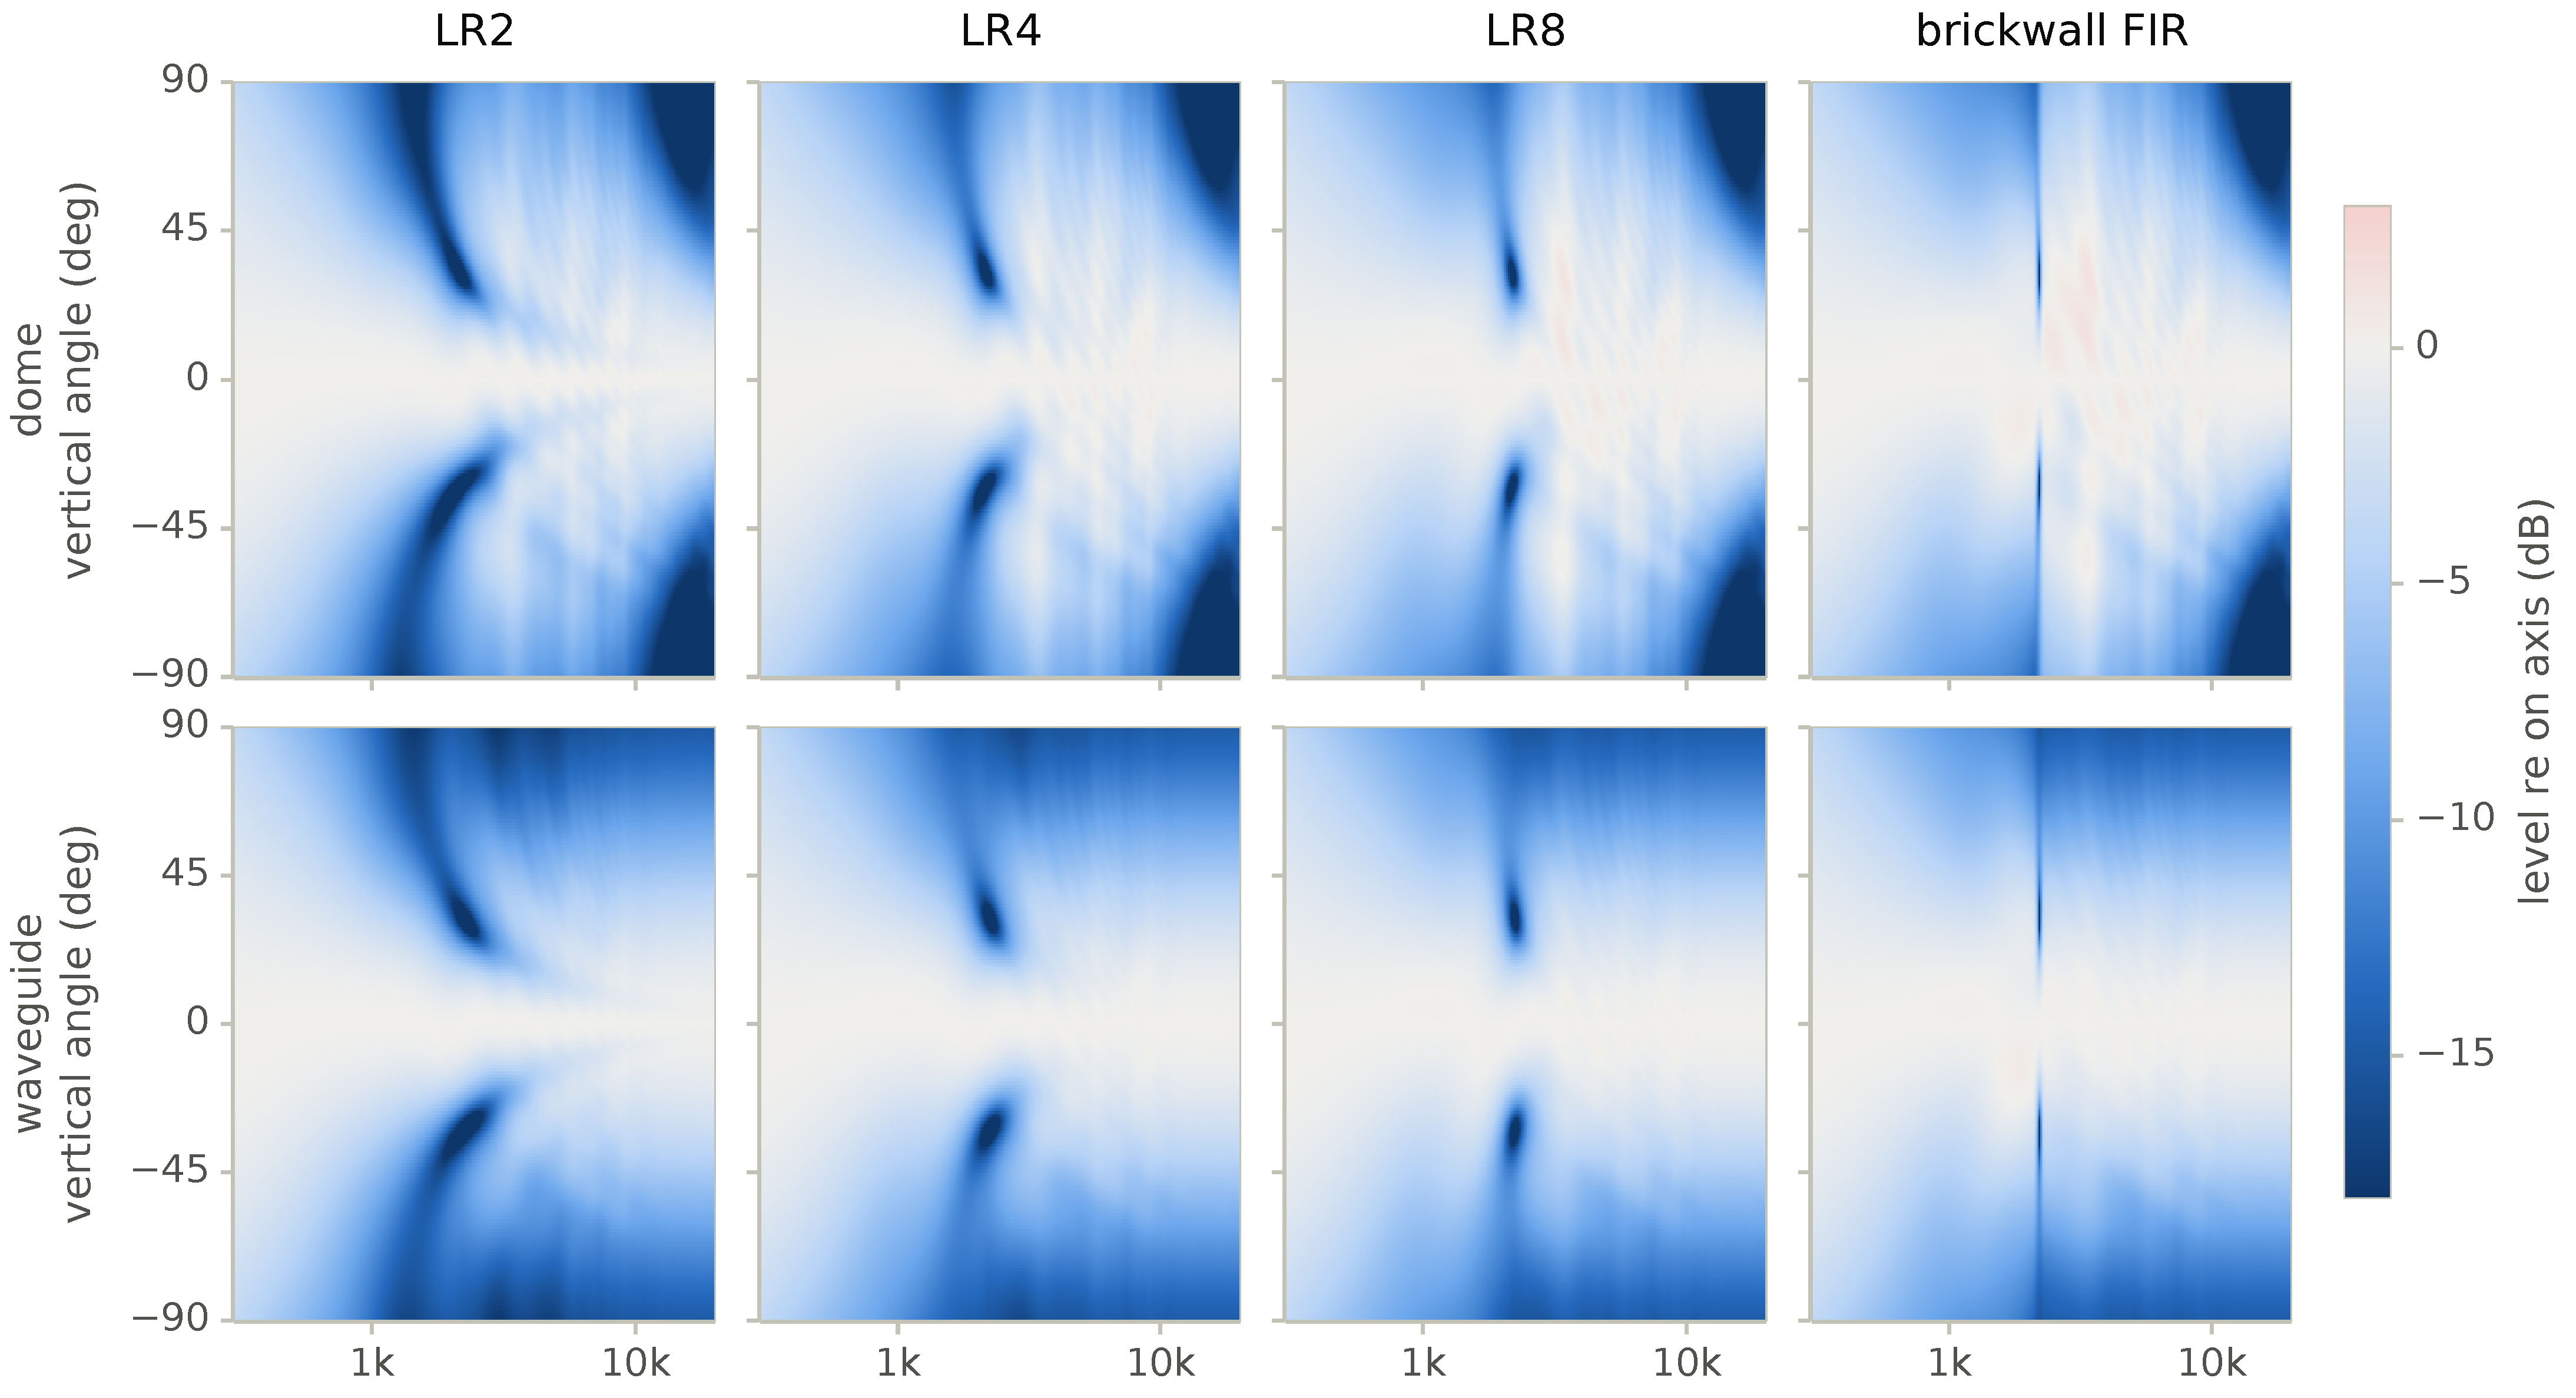
\includegraphics[width=\textwidth]{polar_maps}
\caption{Vertical-plane directivity of the two-way, relative to the on-axis response, with the four
crossovers: plain dome (top), dome in a waveguide (bottom).}
\label{fig:polar}
\end{figure}

% =============================================================================================
\section{The rooms}
\label{sec:rooms}

\subsection{Model}

The rooms are shoeboxes. In the room's frame $x$ runs across the room, $y$ from the wall behind the
listener to the wall behind the loudspeakers, $z$ up. The sound reaching the listener is split three
ways, all in energy.

\paragraph{Specular images} up to the third order \cite{allen1979}. On each axis, with walls at 0 and
$L$, the image of the source $s$ is $u = 2nL + (1 - 2q)s$ ($n$ an integer, $q \in \{0, 1\}$), having
bounced $|n - q|$ times on the wall at 0 and $|n|$ times on the wall at $L$. The loudspeaker emits
that path in the direction $\vect P(\vect r - \vect u)/|\vect r - \vect u|$, $\vect P$ flipping the
axes with an odd number of bounces ($q = 1$), $\vect r$ the listener's head. Its weight is
\begin{equation}
W = \frac{e^{-m |\vect r - \vect u|}}{|\vect r - \vect u|^2}\,\prod_{\text{bounces}} (1 - \alpha)(1 - s),
\end{equation}
$\alpha$ the absorption coefficient, $s$ the scattering coefficient (the share of the reflected energy
sent in all directions instead of the specular one), $m$ the energy attenuation per metre of the air
\cite{iso9613}, and of the furniture beyond the first order.

\paragraph{Diffuse field.} A ray launched from the loudspeaker in direction $\Omega$ is traced through
the box. At each of its first three bounces the scattered share $(1 - \alpha)s$ of the energy it
carries joins a diffuse field; after the third, everything left does. This defines
$g(\Omega) \in [0, 1]$, the share of the energy emitted in direction $\Omega$ that feeds the diffuse
field. In steady state that field gives everywhere
\begin{equation}
p^2_{\mathrm{diff}} = \frac{4}{A}\oint g(\Omega)\,P(\Omega)\dd\Omega, \qquad
A = -S\ln(1 - \bar\alpha) + 4 m V,
\end{equation}
with the Eyring absorption area of the whole room, air and furniture included \cite{kuttruff2016}.
With $g = 1 - \alpha$ everywhere this is the room term $4/R$ of Hopkins and Stryker
\cite{hopkins1948}. The integral runs over 3000 directions of a Fibonacci lattice.

\paragraph{Direct sound,} the image of order 0.

Absorbing patches (a rug, panels, a ceiling cloud) replace a surface's coefficients where a ray or a
first-order reflection lands on them; the higher-order images and the diffuse field use each
surface's area-weighted mean. The furniture is an equivalent absorption area $A_f$ spread over the
volume, an attenuation $m_f = A_f / 4V$ per metre applied to the images of order 2 and more, to the rays
and to the diffuse field; the direct sound and the first reflections are assumed unobstructed.

The energy at the listener is then
\begin{equation}
E(f) = \sum_{\text{images}} W_k(f)\,P(\Omega_k, f) + \sum_{\text{lattice}} \frac{4}{A}\,\frac{4\pi}{N}\,g(\Omega_l, f)\,P(\Omega_l, f),
\end{equation}
a set of weights over directions, like the standard's curves. We give it relative to an
omnidirectional source at the same place ($P \equiv 1$), which divides out the room's own colouration
(its absorption rising with frequency): $E(f) / E_{\mathrm{omni}}(f)$ is how the room weighs the
loudspeaker's directions, the quantity the PIR estimates. A loudspeaker radiating the same everywhere
gets 0\,dB in every room. Two versions: the \emph{steady state}, every path, and the \emph{early
sound}, the direct sound and the six first reflections, what the LW and the ER stand for.

\subsection{Checks}

In a room with uniform absorption the model agrees with Hopkins--Stryker when every reflection
scatters ($s = 1$), within 1\,\%. When none does ($s = 0$), its total energy is within 3 to 7\,\%
(0.15 to 0.3\,dB) of a full image method summed to the 26th or 40th order (25\,000 and 88\,000
images), for $\bar\alpha = 0.25$ and 0.1. The rooms' scattering coefficients (0.05 to 0.5) lie
between these two cases.

\subsection{The ensemble}

Each setup holds the left loudspeaker of a stereo pair and a listener on the room's middle line
(the right loudspeaker is its mirror image). The 300 random setups (table~\ref{tab:ensemble}) draw:
width 3.4--5.2\,m, length 4.5--7.5\,m, height 2.4--2.8\,m; loudspeakers on the short wall, their baffles
0.4--1.2\,m from it, 1.8--2.8\,m apart and at least 0.45\,m from the side walls, the reference axis
0.85--1.15\,m high; listener 2.0--3.8\,m from the baffles' line and at least 0.5\,m in front of the wall
behind, ears 1.0--1.25\,m high; loudspeakers aimed at the listener (half the setups), parallel to the
side walls (a quarter) or halfway (a quarter). Walls of painted plaster on masonry or plasterboard on
studs, one with a window (2--6\,m$^2$) and curtains (0--4\,m$^2$); ceiling of plaster or plasterboard;
floor of parquet or tiles (60\,\%, half of them with a rug $2$--$3 \times 2.5$--$3.5$\,m in front of the
loudspeakers) or wall-to-wall carpet; furniture absorbing 6--16\,m$^2$ at 1\,kHz, half that at
125\,Hz. A quarter of the rooms (\ntreated) is treated: panels of 50\,mm mineral wool, $1.2 \times
1.2$\,m, at the side walls' first reflection points, and a rug; their ceilings stay bare. The
absorption and scattering coefficients are typical textbook values; the reverberation times
(\nrtMedian\,s median at 1\,kHz, \nrtLo--\nrtHi\,s for 80\,\% of the rooms) fall in the range measured in
furnished dwellings \cite{diaz2005}. The first 150 rooms fit the updated weights, the other 150 test
them.

\begin{table}[t]
\centering
\caption{The 300 random setups: 10th percentile, median, 90th percentile.}
\label{tab:ensemble}
\begin{tabular}{lrrr}
\toprule
& 10\,\% & median & 90\,\% \\
\midrule
\rows{ensemble}
\bottomrule
\end{tabular}
\end{table}

\begin{figure}[t]
\centering
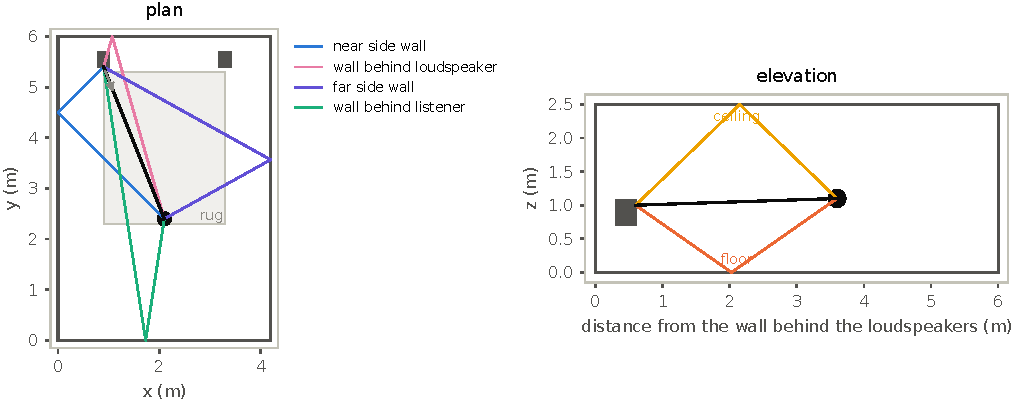
\includegraphics[width=\textwidth]{setup}
\caption{One of the rooms ($4.2 \times 6.0 \times 2.5$\,m, parquet and rug): the left loudspeaker, the
listener, the direct sound (black) and the six first reflections.}
\label{fig:setup}
\end{figure}

% =============================================================================================
\section{The standard against the rooms}
\label{sec:standard}

\subsection{Where the energy goes}

For an omnidirectional source, the direct sound brings \ndirectShare\,\% of the steady-state energy at
1\,kHz (median), the six first reflections \nfirstShare\,\% together, the later paths \nlateShare\,\%
(table~\ref{tab:shares}, figure~\ref{fig:shares}). The PIR gives 12\,\% to the Listening Window, 44\,\%
to the Early Reflections and 44\,\% to the Sound Power: about twice the direct sound's share and four
times the first reflections'.

Among the first reflections the floor and the ceiling bring \nvertShare\,\% of the energy
(\nvertLo--\nvertHi\,\%), the side walls \nsideShare\,\%: the share the Early Reflections give them,
two bounces of five. In the treated rooms the floor and ceiling rise to \nvertTreated\,\% (\nvertUntreated\,\%
in the others). The ceiling outweighs the floor: rugs and carpets absorb the floor bounce, and the
furniture on the floor scatters it.

\begin{table}[t]
\centering
\caption{Share of the energy at the listener (\%), omnidirectional source: median and 10--90\,\%
range over the 300 rooms.}
\label{tab:shares}
\begin{tabular}{lrrrr}
\toprule
& \multicolumn{2}{c}{1\,kHz} & \multicolumn{2}{c}{4\,kHz} \\
& median & range & median & range \\
\midrule
\rows{shares}
\bottomrule
\end{tabular}
\end{table}

\begin{figure}[t]
\centering
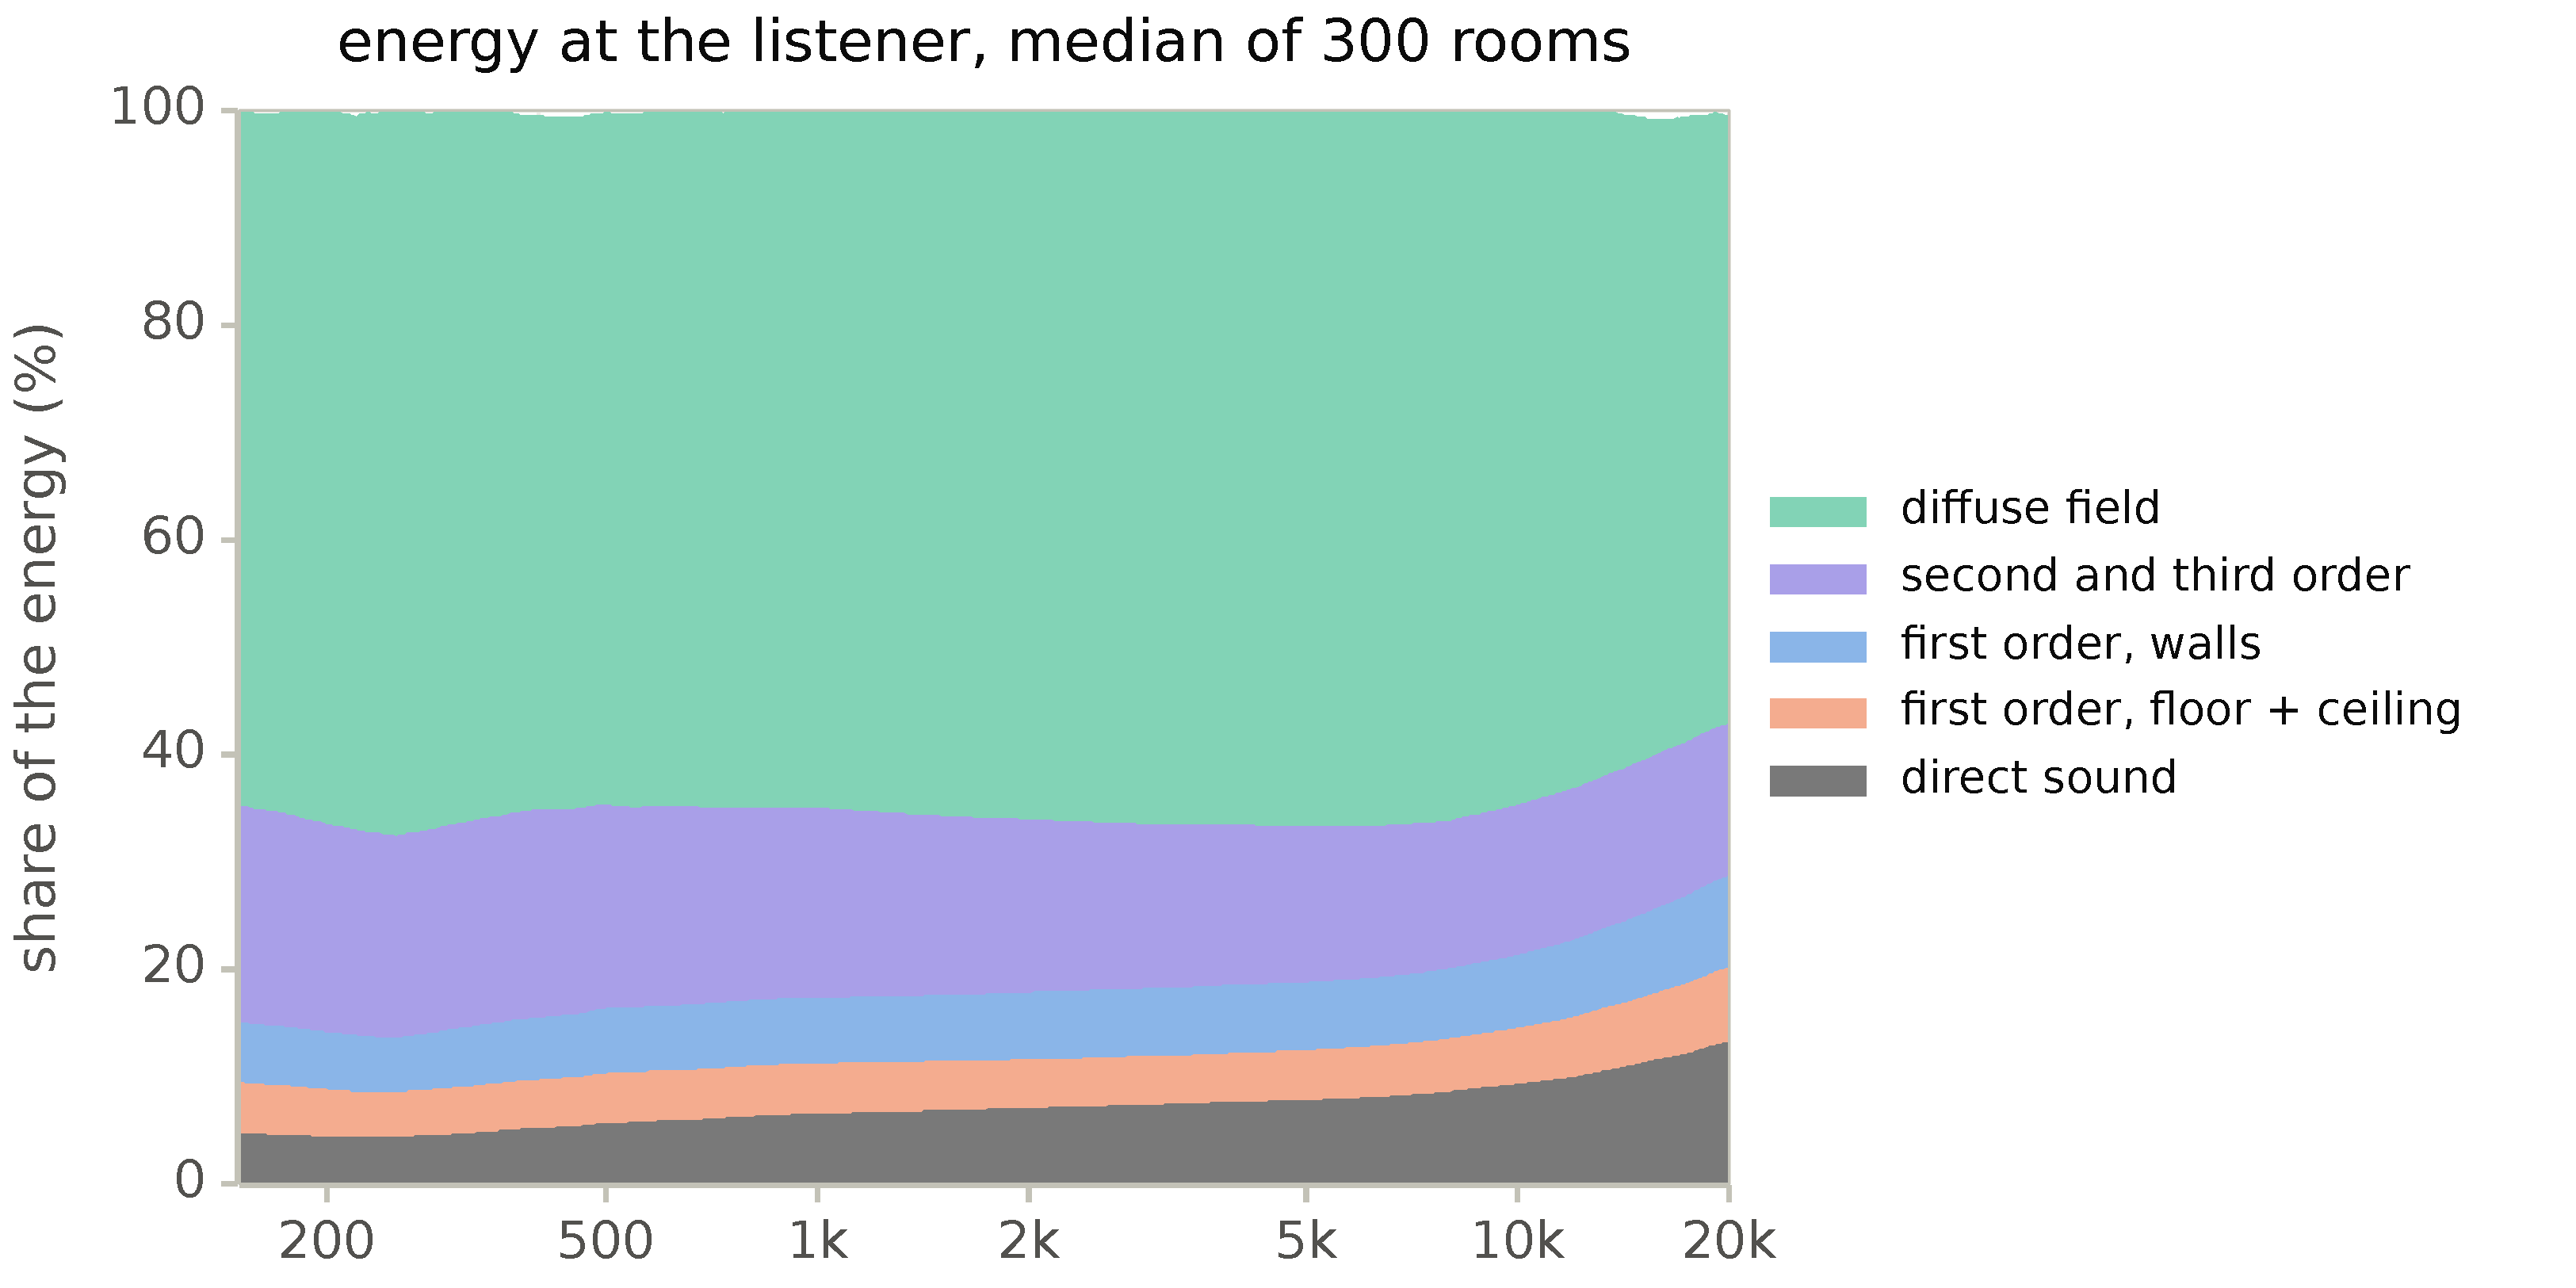
\includegraphics[width=0.75\textwidth]{shares}
\caption{Share of the energy at the listener by kind of path, omnidirectional source, median of the
300 rooms.}
\label{fig:shares}
\end{figure}

\subsection{In which directions}

The first reflections leave the loudspeaker where the standard looks for them
(table~\ref{tab:directions}, figures~\ref{fig:kernels} and~\ref{fig:angles}). The floor bounce leaves
at $\nangleFloor^\circ$ (median), the ceiling bounce at $\nangleCeiling^\circ$; the standard's floor and
ceiling angles bracket them, its $-20^\circ$ and $60^\circ$ fitting listeners farther or closer than
these. Both arrive first, \ndelayFloor\ and \ndelayCeiling\,ms after the direct sound, with the near
side wall (\ndelayLeft\,ms): in rooms wider than high the floor and ceiling are the nearest surfaces.
The side walls fall within the standard's $\pm40$ to $\pm80^\circ$; the wall behind the listener (the
standard's front wall) within its $\pm30^\circ$. The wall behind the loudspeakers (its rear wall) is
reached at $137$ to $166^\circ$, where the standard looks at $\pm90^\circ$ and $180^\circ$.

\begin{table}[t]
\centering
\caption{Directions in which the first reflections leave the loudspeaker (degrees, median and
10--90\,\% range over the 300 rooms), the standard's angles (V vertical, H horizontal orbit) and the
reflections' delay after the direct sound (median).}
\label{tab:directions}
\small
\begin{tabular}{llrrlr}
\toprule
reflection & angle & median & range & CTA-2034 & delay (ms) \\
\midrule
\rows{directions}
\bottomrule
\end{tabular}
\end{table}

\begin{figure}[t]
\centering
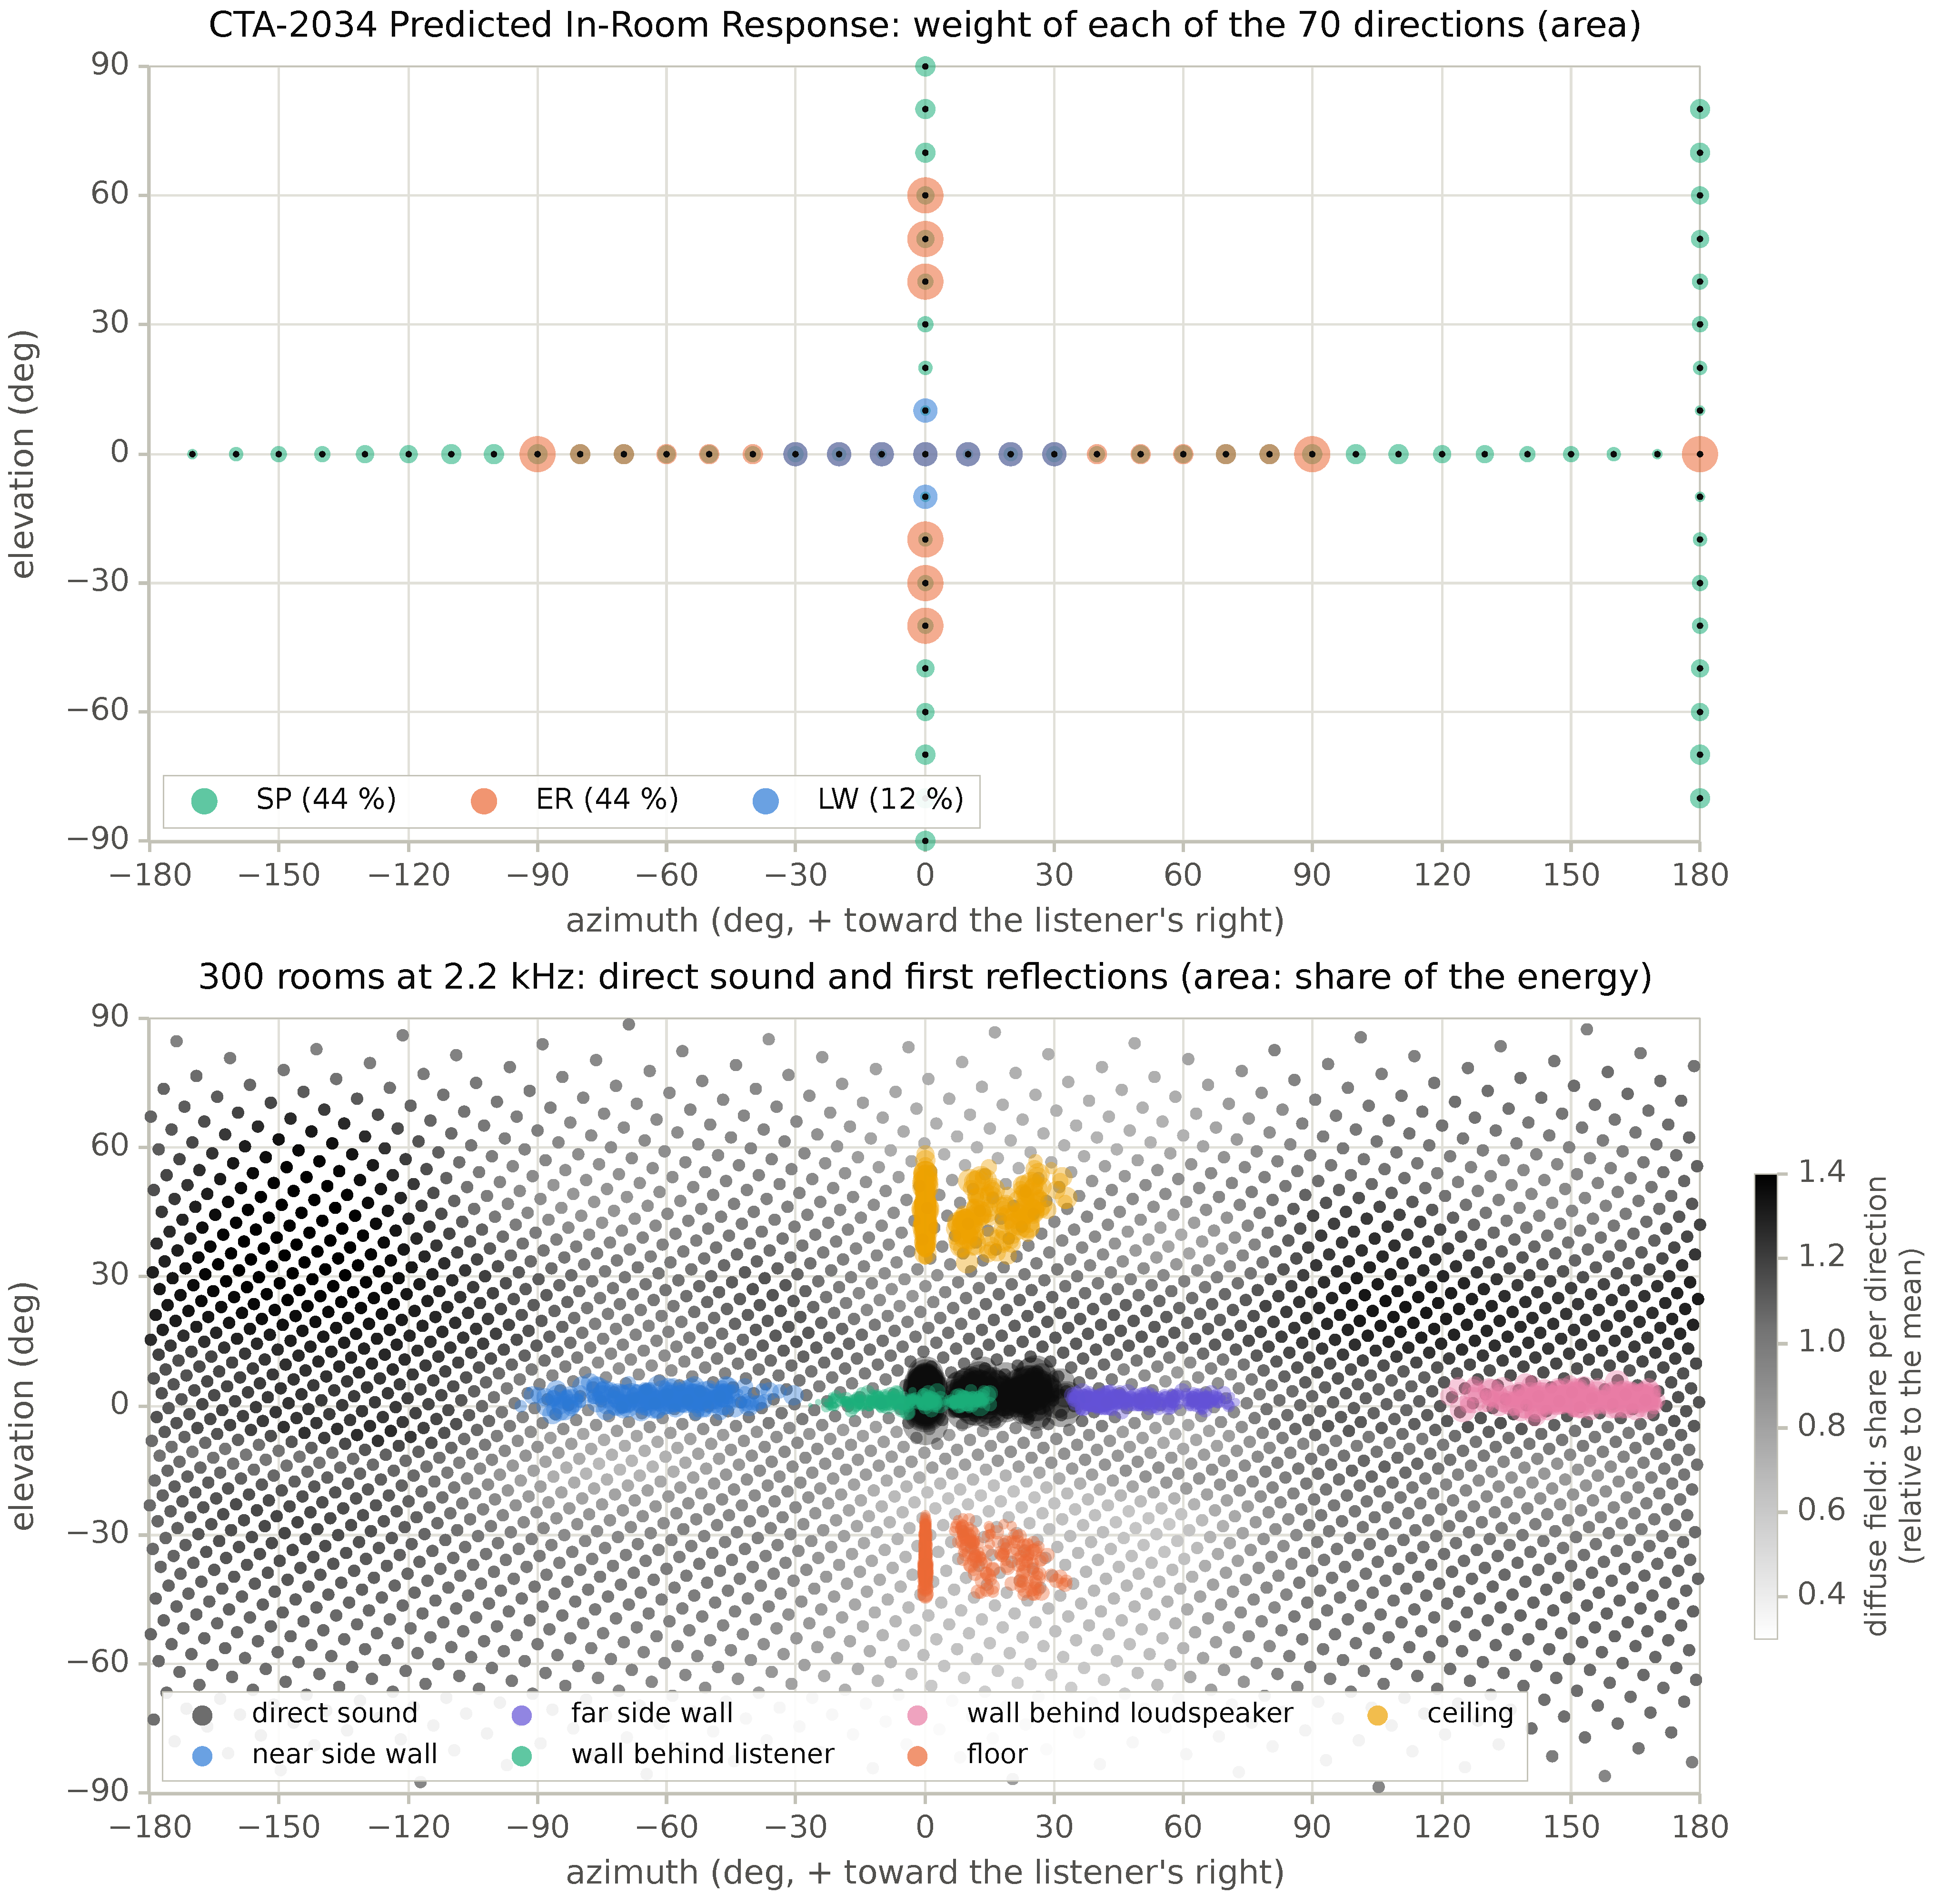
\includegraphics[width=\textwidth]{kernel_maps}
\caption{Top: the weight the PIR gives each of the 70 directions (area of the circles), split into its
LW, ER and SP parts; beyond $90^\circ$ the vertical orbit is drawn at azimuth $180^\circ$. Bottom: the
300 rooms at 2.2\,kHz, the direct sound and the first reflections (area: share of the energy at the
listener), over the diffuse field's share per direction $g$, relative to its mean (grey).}
\label{fig:kernels}
\end{figure}

\begin{figure}[t]
\centering
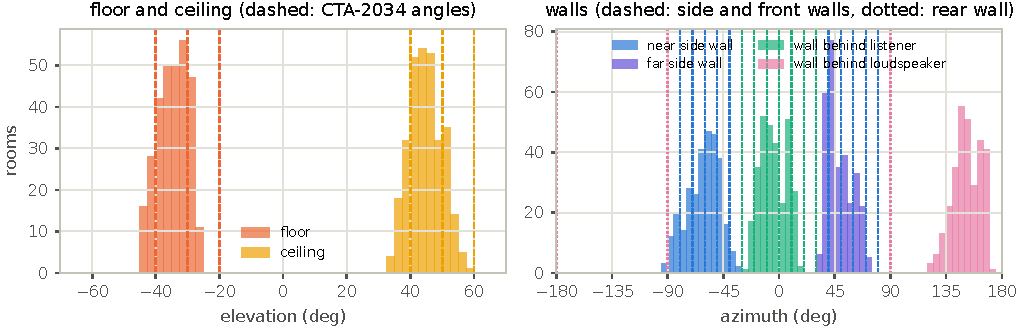
\includegraphics[width=\textwidth]{reflection_angles}
\caption{Directions of the first reflections in the 300 rooms, and the standard's angles.}
\label{fig:angles}
\end{figure}

The diffuse field does not draw evenly on all directions either (figure~\ref{fig:kernels}, bottom):
what the loudspeaker sends toward an absorbing floor or a rug feeds it less than what it sends
backward or upward. The differences reach about $\pm30$\,\%, much less than the standard's contrast
between the ER directions and the rest.

\subsection{Predicting the in-room response}
\label{sec:prediction}

With weights summing to one fitted on the 150 training rooms, all sixteen loudspeaker variants together,
the steady-state response is best predicted by
\begin{equation}
\nwLw\,\mathrm{LW} + \nwEr\,\mathrm{ER} + \nwSp\,\mathrm{SP}_{\mathrm{sphere}},
\end{equation}
with the sound power integrated over the sphere, or by $\nwLwTwo\,\mathrm{LW} + \nwErTwo\,\mathrm{ER} +
\nwSpTwo\,\mathrm{SP}$ with the two orbits' (table~\ref{tab:errors}, figure~\ref{fig:errors}). Fitted to
subsets (treated rooms, reverberation times below 0.33 or above 0.5\,s, listeners closer than 2.6 or
farther than 3.2\,m), the LW weight stays between 0.07 and 0.16 and the ER weight between $-0.05$ and
0.04. Fitted on the plain dome alone, the weights predict the waveguide as well as its own fit. The
Early Reflections do not help: their directions are those of a minor share of the energy, which the
LW and SP already describe. On the test rooms these weights are as close to each room as the mean of
the training rooms is, the room-to-room floor. The PIR is 1.7 to 2.1\,dB RMS off, mostly by a bias: it
sits \npirBiasLow\,dB above the rooms at 300\,Hz and up to \npirBiasMax\,dB above at the crossover,
because it leans on the Listening Window, where a forward-directional loudspeaker is loudest
(figure~\ref{fig:spin}).

For the early sound alone the rooms weigh about $\nwLwEarly\,\mathrm{LW} + \nwErEarly\,\mathrm{ER} +
\nwSpEarly\,\mathrm{SP}$: the direct sound brings \nearlyDirect\,\% of it, where the early part of the PIR
($0.12\,\mathrm{LW} + 0.44\,\mathrm{ER}$, normalized) gives the Listening Window 21\,\%.

\begin{table}[t]
\centering
\caption{Predicting the steady-state response of the 150 test rooms, 300\,Hz--16\,kHz: median RMS
error over the rooms, and largest mean error (bias) over frequency, range over the sixteen
variants (dB).}
\label{tab:errors}
\begin{tabular}{lrr}
\toprule
prediction & RMS error & largest bias \\
\midrule
\rows{errors}
\bottomrule
\end{tabular}
\end{table}

\begin{figure}[t]
\centering
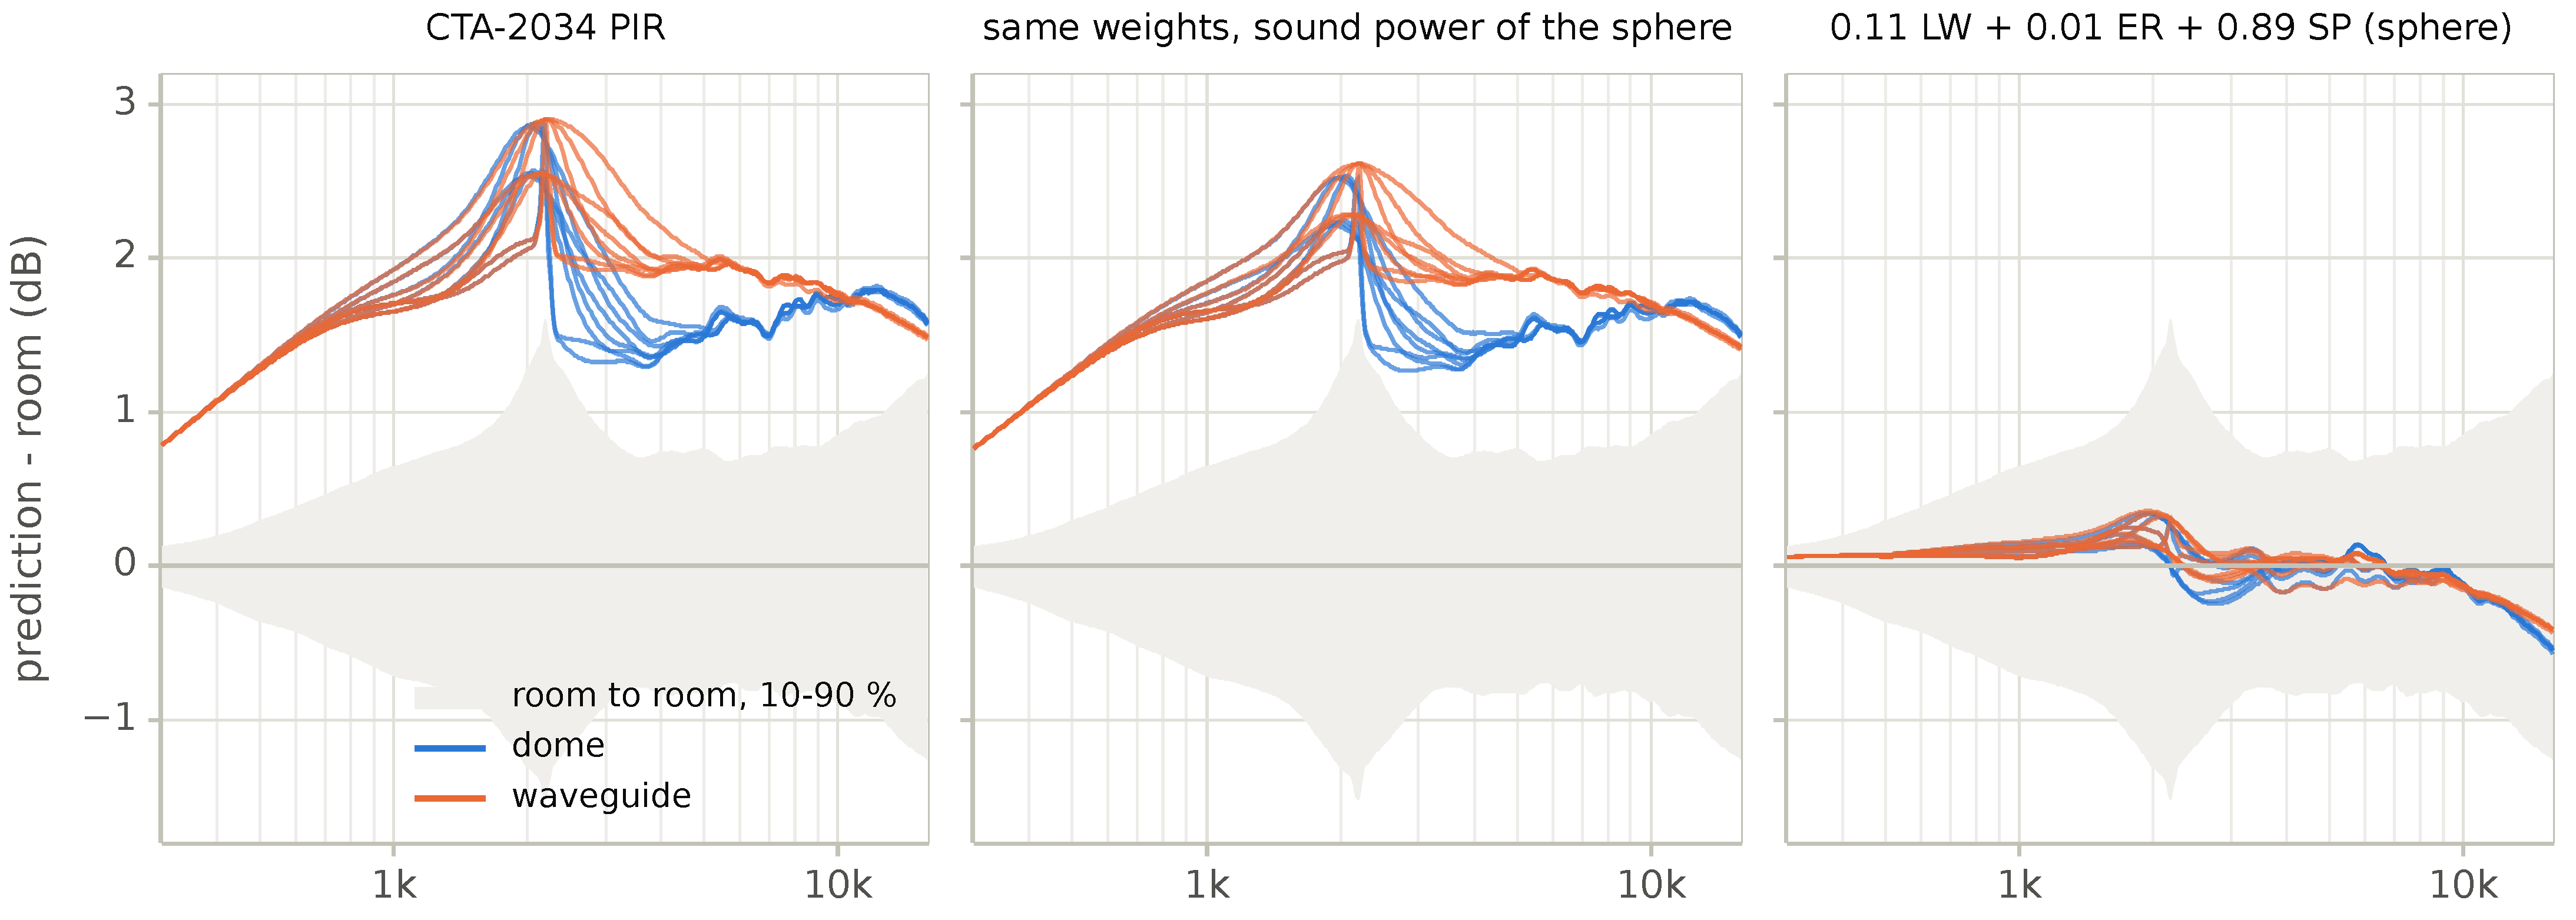
\includegraphics[width=\textwidth]{errors}
\caption{Mean error of three predictions on the 150 test rooms, every variant (thin lines), and the
rooms' own spread around their mean (grey).}
\label{fig:errors}
\end{figure}

\begin{figure}[t]
\centering
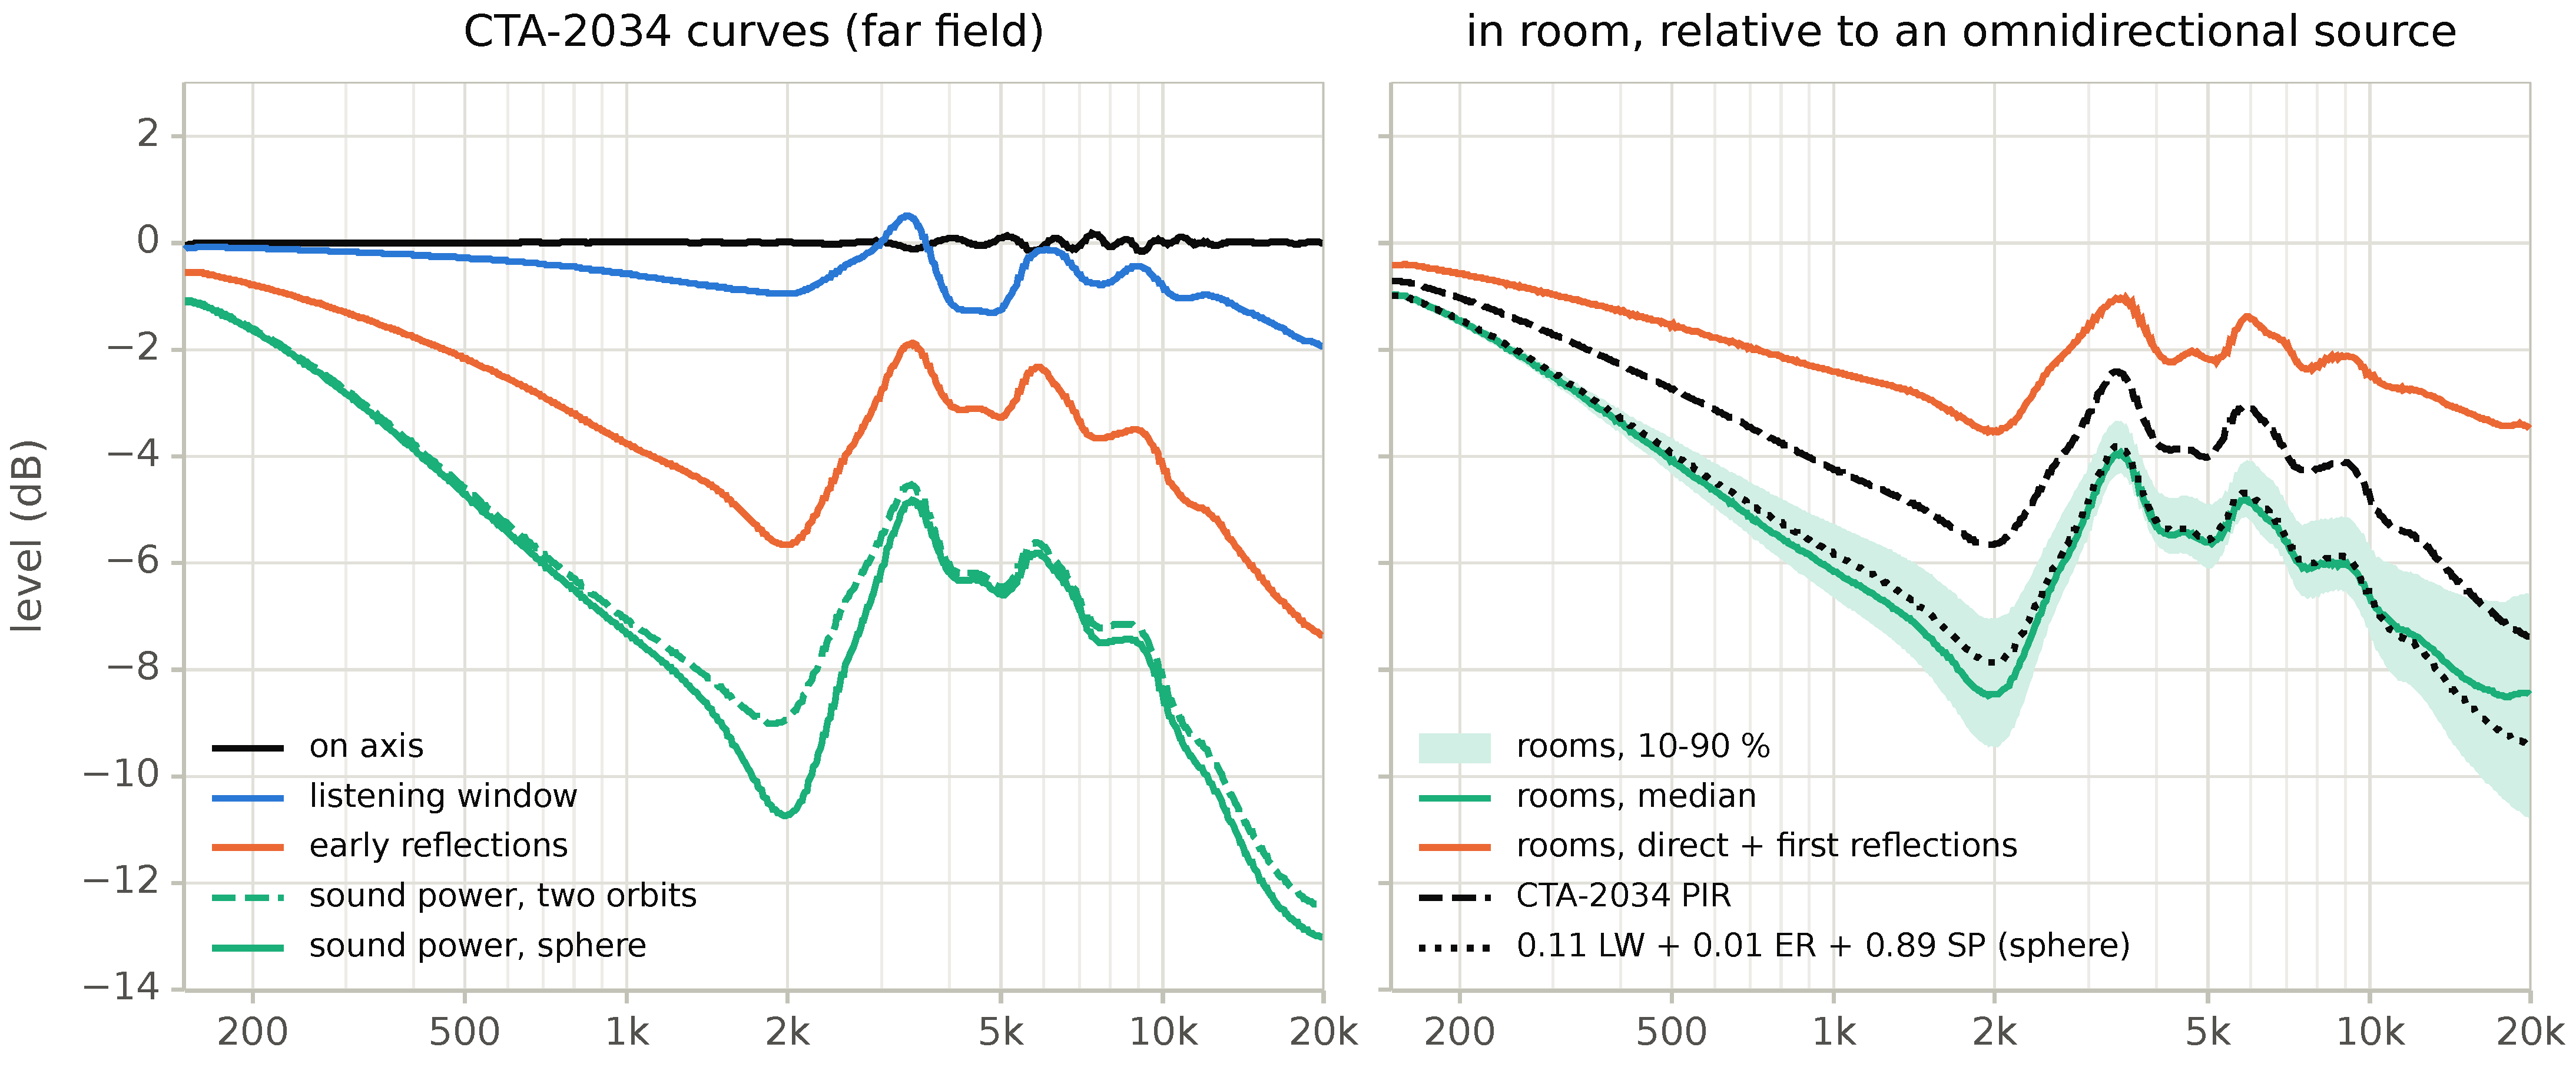
\includegraphics[width=\textwidth]{spin_dome}
\caption{The upright two-way, plain dome, LR4. Left: its CTA-2034 curves, the sound power from two
orbits and over the sphere. Right: in the rooms, relative to an omnidirectional source, steady state
(median and 10--90\,\% range) and early sound (median), with the PIR and the fitted weights.}
\label{fig:spin}
\end{figure}

\subsection{The sound power from two orbits}
\label{sec:sp}

Around the crossover both drivers play, and the lobing between them costs sound power. The upright
loudspeaker's horizontal orbit sees no interference, the drivers being at the same distance from it;
the vertical orbit sees it. The two orbits get the same weight, where only a thin band of the sphere
around the horizontal plane is spared. At 2\,kHz the two-orbit sound power is \nspBiasLrFour\,dB too high
with LR4 (\nspBiasLrTwo\ with LR2, \nspBiasLrEight\ with LR8; figure~\ref{fig:sporbits}): of the 2.6\,dB by
which the LR4's sound power falls below the brickwall's there, the two orbits show 1.2. The same
happens on its side, the orbits trading roles. Above the crossover the two orbits overestimate the
directional dome by 0.2 to 0.6\,dB, the effect of the spherical squares (section~\ref{sec:cta}).

\begin{figure}[t]
\centering
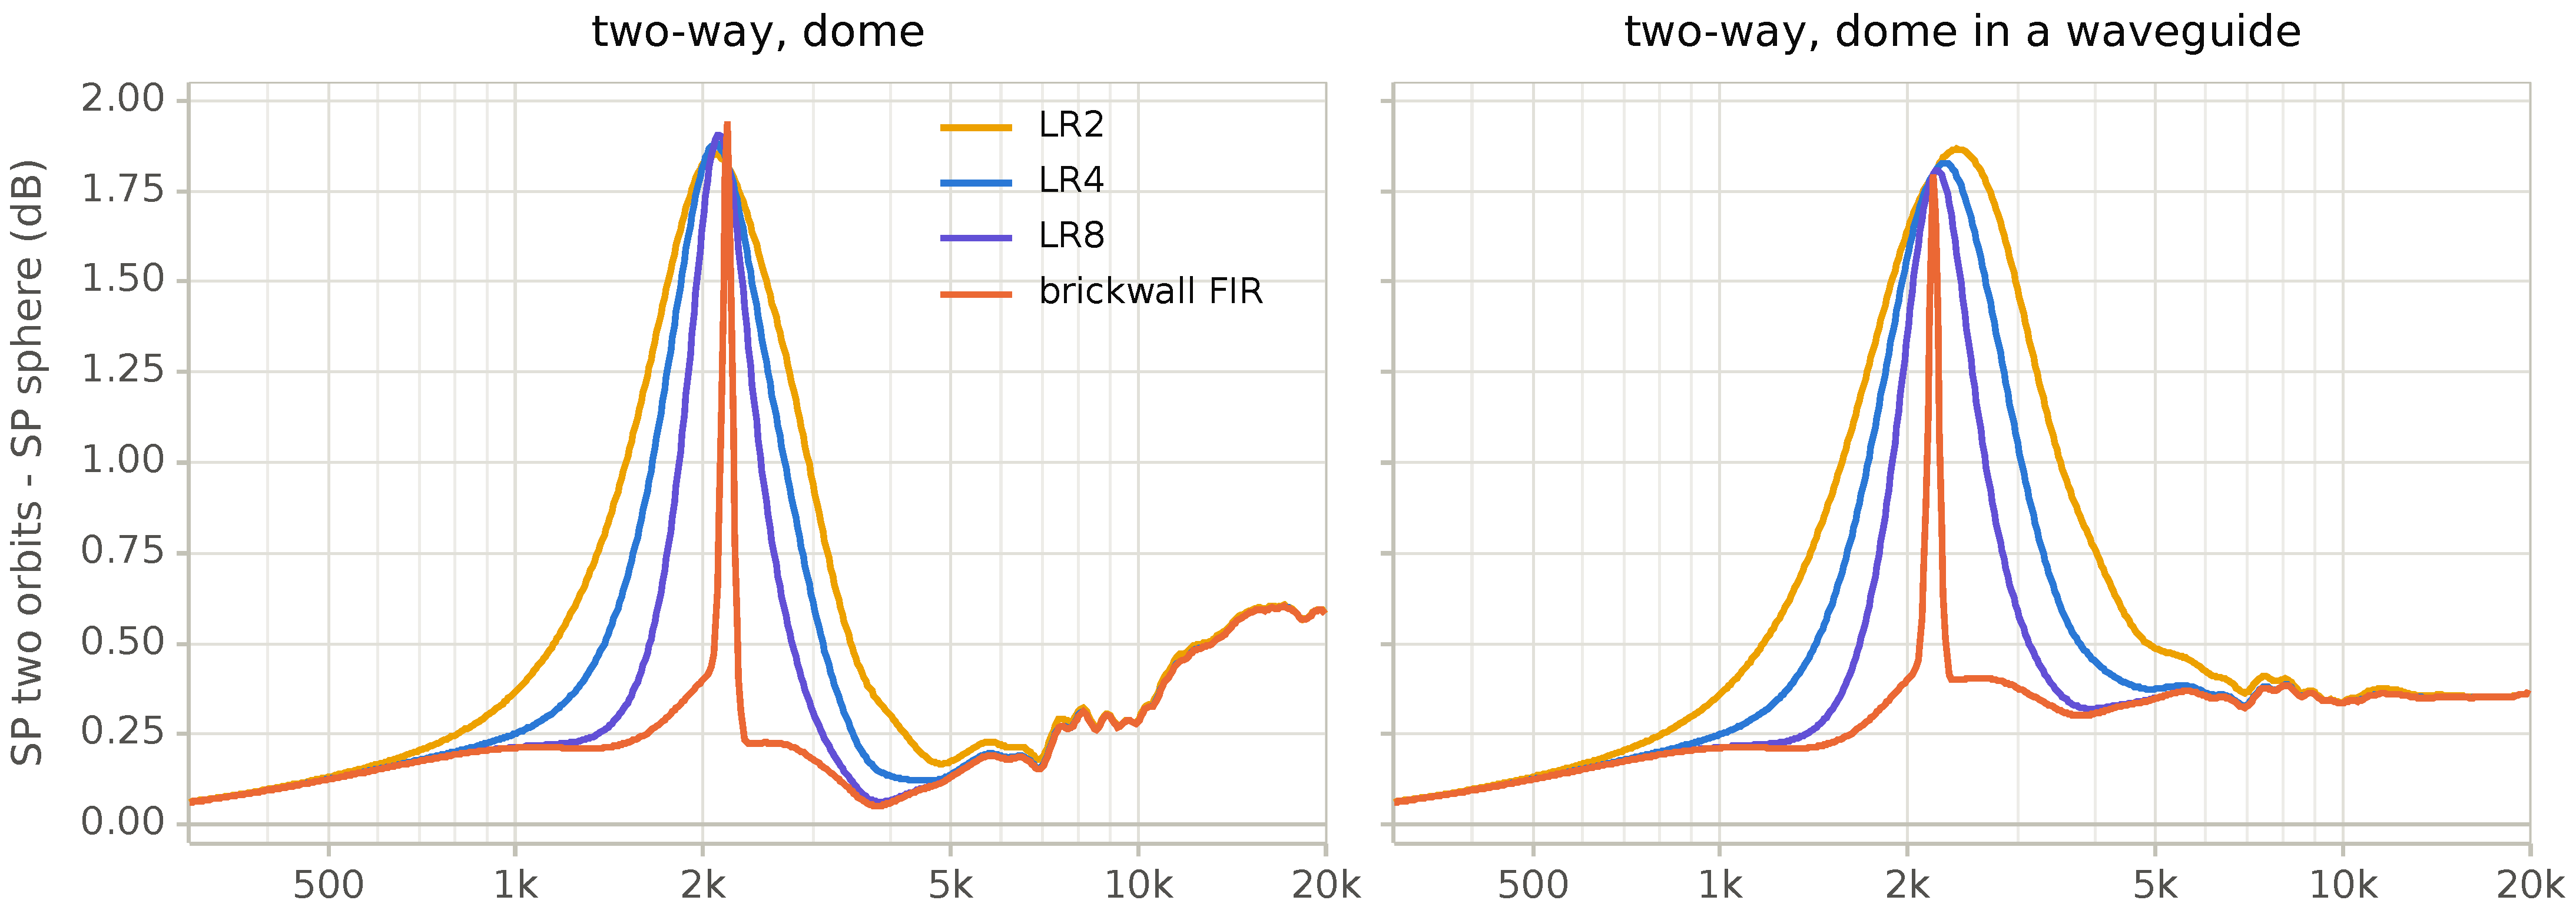
\includegraphics[width=\textwidth]{sp_orbits}
\caption{Sound power from the two orbits minus the sound power over the sphere, upright two-way.}
\label{fig:sporbits}
\end{figure}

\subsection{Upright or on its side}

Laid on its side, the loudspeaker lobes horizontally instead of vertically. The Listening Window sees
the difference (figure~\ref{fig:rotation}): about 1\,dB down at 2\,kHz upright, 2.3 to 2.6\,dB on its side;
the PIR barely moves. The rooms' steady state does not move either: it is mostly sound power, which
does not depend on the orientation. The early sound does, though not in its median. Upright, no room
leaves the listener more than 1.1\,dB below the median at the crossover; on its side, a quarter of
the rooms leave the listener more than 3\,dB below it, one in ten 5.7\,dB: setups where the
loudspeakers are not aimed at the listener, who sits 23 to $33^\circ$ off axis, near the lobing's first
null ($34^\circ$ at 2.2\,kHz). Seated listeners hear the direct sound within $5^\circ$ of the axis vertically (90\,\% of the
rooms), and up to $24^\circ$ horizontally. The Listening Window's $\pm30^\circ$ horizontally and
$\pm10^\circ$ vertically follow that asymmetry. The vertical lobing reaches the listener through the
floor and ceiling bounces and the reverberant field, which the ER and the SP carry, averaged
(section~\ref{sec:crossovers}).

\begin{figure}[t]
\centering
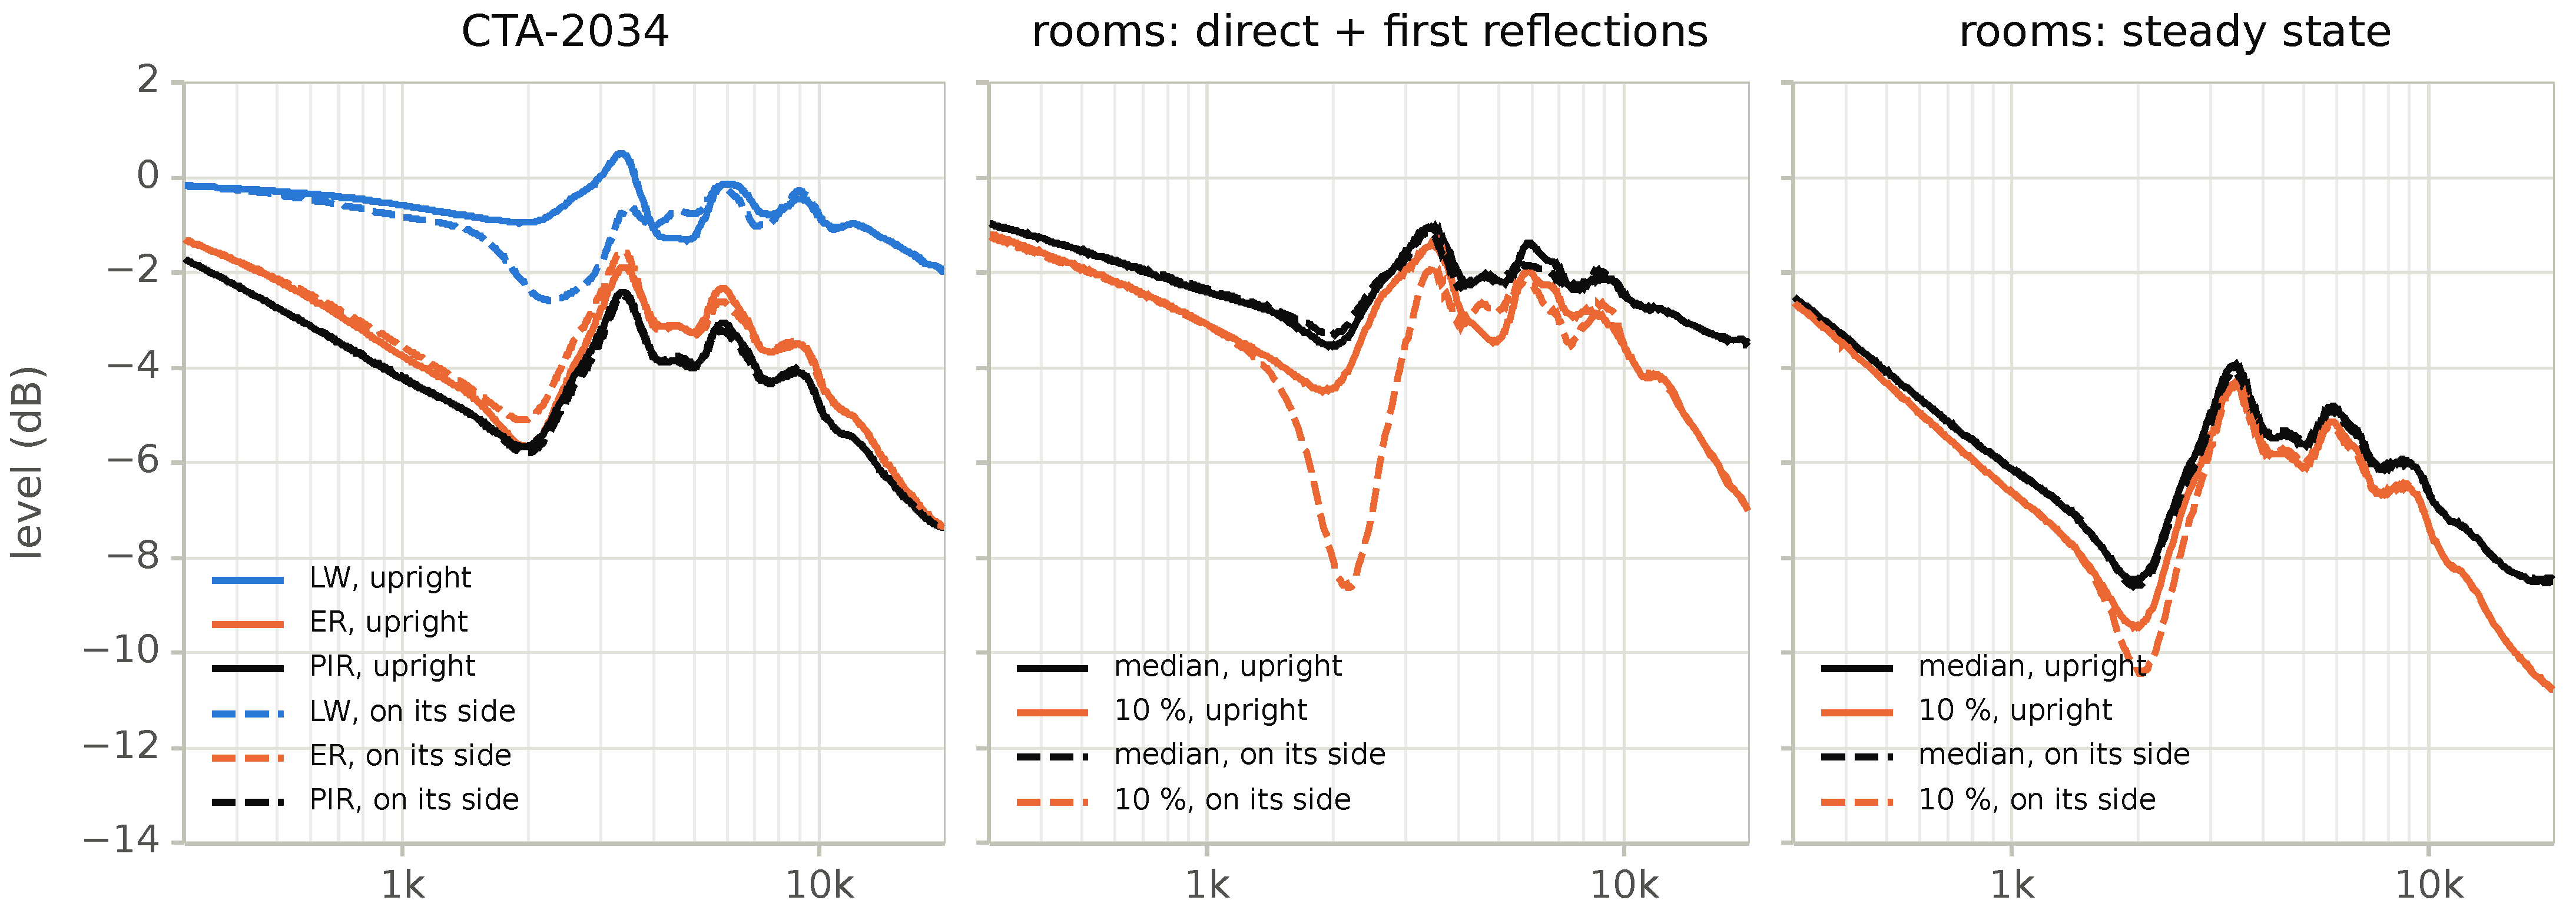
\includegraphics[width=\textwidth]{rotation}
\caption{The two-way with LR4, upright and on its side. Left: its LW, ER and PIR. Middle and right: the
rooms, early sound and steady state, median and 10th percentile.}
\label{fig:rotation}
\end{figure}

% =============================================================================================
\section{Linkwitz-Riley against brickwall FIR}
\label{sec:crossovers}

\subsection{Averages and paths}

A crossover's defects lie within about an octave of its frequency, and in each direction at a
frequency of its own: two drivers $d$ apart cancel where $d \sin\theta$ is half a wavelength, at
$34^\circ$ for 2.2\,kHz and 140\,mm, at wider angles for lower frequencies. Adding directions in
power, as the in-room curve, the PIR and every curve of the standard do, adds notches that fall at
different frequencies, and fills them. Two measures follow.

\emph{Averaged curve.} The deviation of a curve (dB against log frequency) from the straight line that
best fits it from 600\,Hz to 8\,kHz, a loudspeaker whose directivity index rises evenly giving a
straight line; its RMS within one octave of the crossover (1.1 to 4.4\,kHz), and the deepest dip there.

\emph{Colouration of the paths.} The same deviation for the response in each direction, before any
averaging, then weighted by the energy that path brings to the listener: the room's weight times the
loudspeaker's power in that direction, averaged over 600\,Hz--8\,kHz and over the four crossovers. The
weights are thus the same for all crossovers, so that a notch does not lower the weight of the path it
colours. Groups: every path (steady state), the first reflections, the floor and ceiling bounces alone;
and the 70 directions with the PIR's weights or the updated ones.

\subsection{What the floor and ceiling bounces carry}

\begin{figure}[t]
\centering
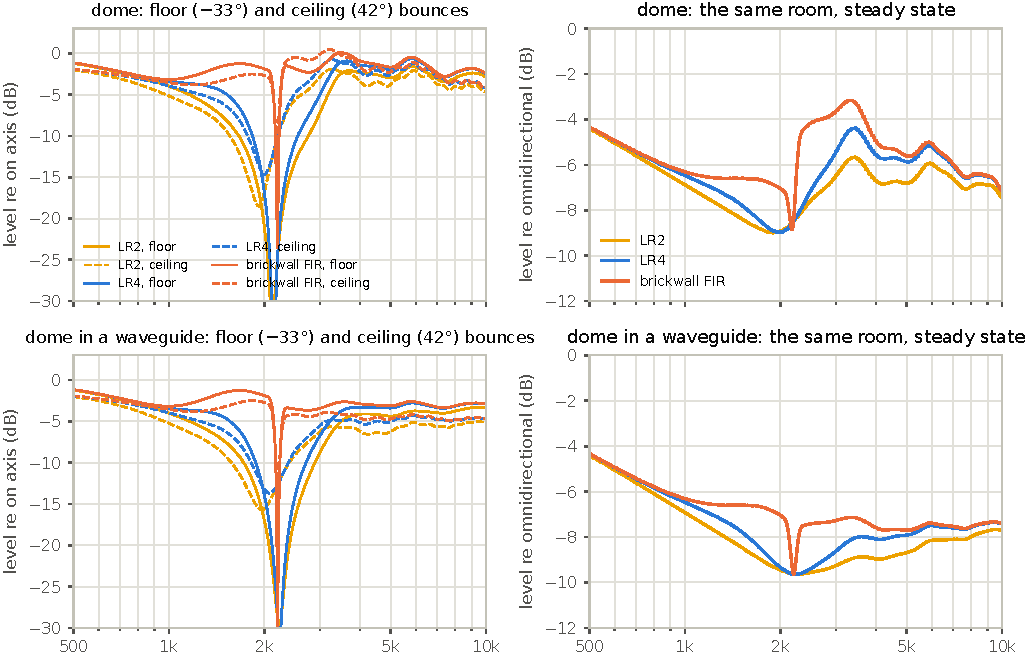
\includegraphics[width=\textwidth]{paths}
\caption{The living room of figure~\ref{fig:setup}. Left: the loudspeaker's response in the directions
of the floor and ceiling bounces, relative to the axis, with three crossovers. Right: the same room's
steady-state response, relative to an omnidirectional source.}
\label{fig:paths}
\end{figure}

In the living room of figure~\ref{fig:setup} the floor bounce leaves at $-33^\circ$, close to the first
null, and the ceiling bounce at $+42^\circ$ (figure~\ref{fig:paths}). With the plain dome and LR4, the
floor bounce has a notch \nnotchDomeLrFourFloorDepth\,dB deep, \nnotchDomeLrFourFloorWidth\,Hz wide at
$-6$\,dB from the straight line (\nnotchDomeLrTwoFloorWidth\,Hz with LR2); the brickwall's is
\nnotchDomeFirFloorDepth\,dB deep and \nnotchDomeFirFloorWidth\,Hz wide. At the ceiling, farther from the
null: \nnotchDomeLrFourCeilingDepth\,dB over \nnotchDomeLrFourCeilingWidth\,Hz with LR4,
\nnotchDomeFirCeilingDepth\,dB over \nnotchDomeFirCeilingWidth\,Hz with the brickwall. With the waveguide the
notches are as deep, and the brickwall's as narrow. In the same room's averaged response the LR4 leaves
a dip of 2 to 3\,dB, about an octave wide.

\begin{figure}[t]
\centering
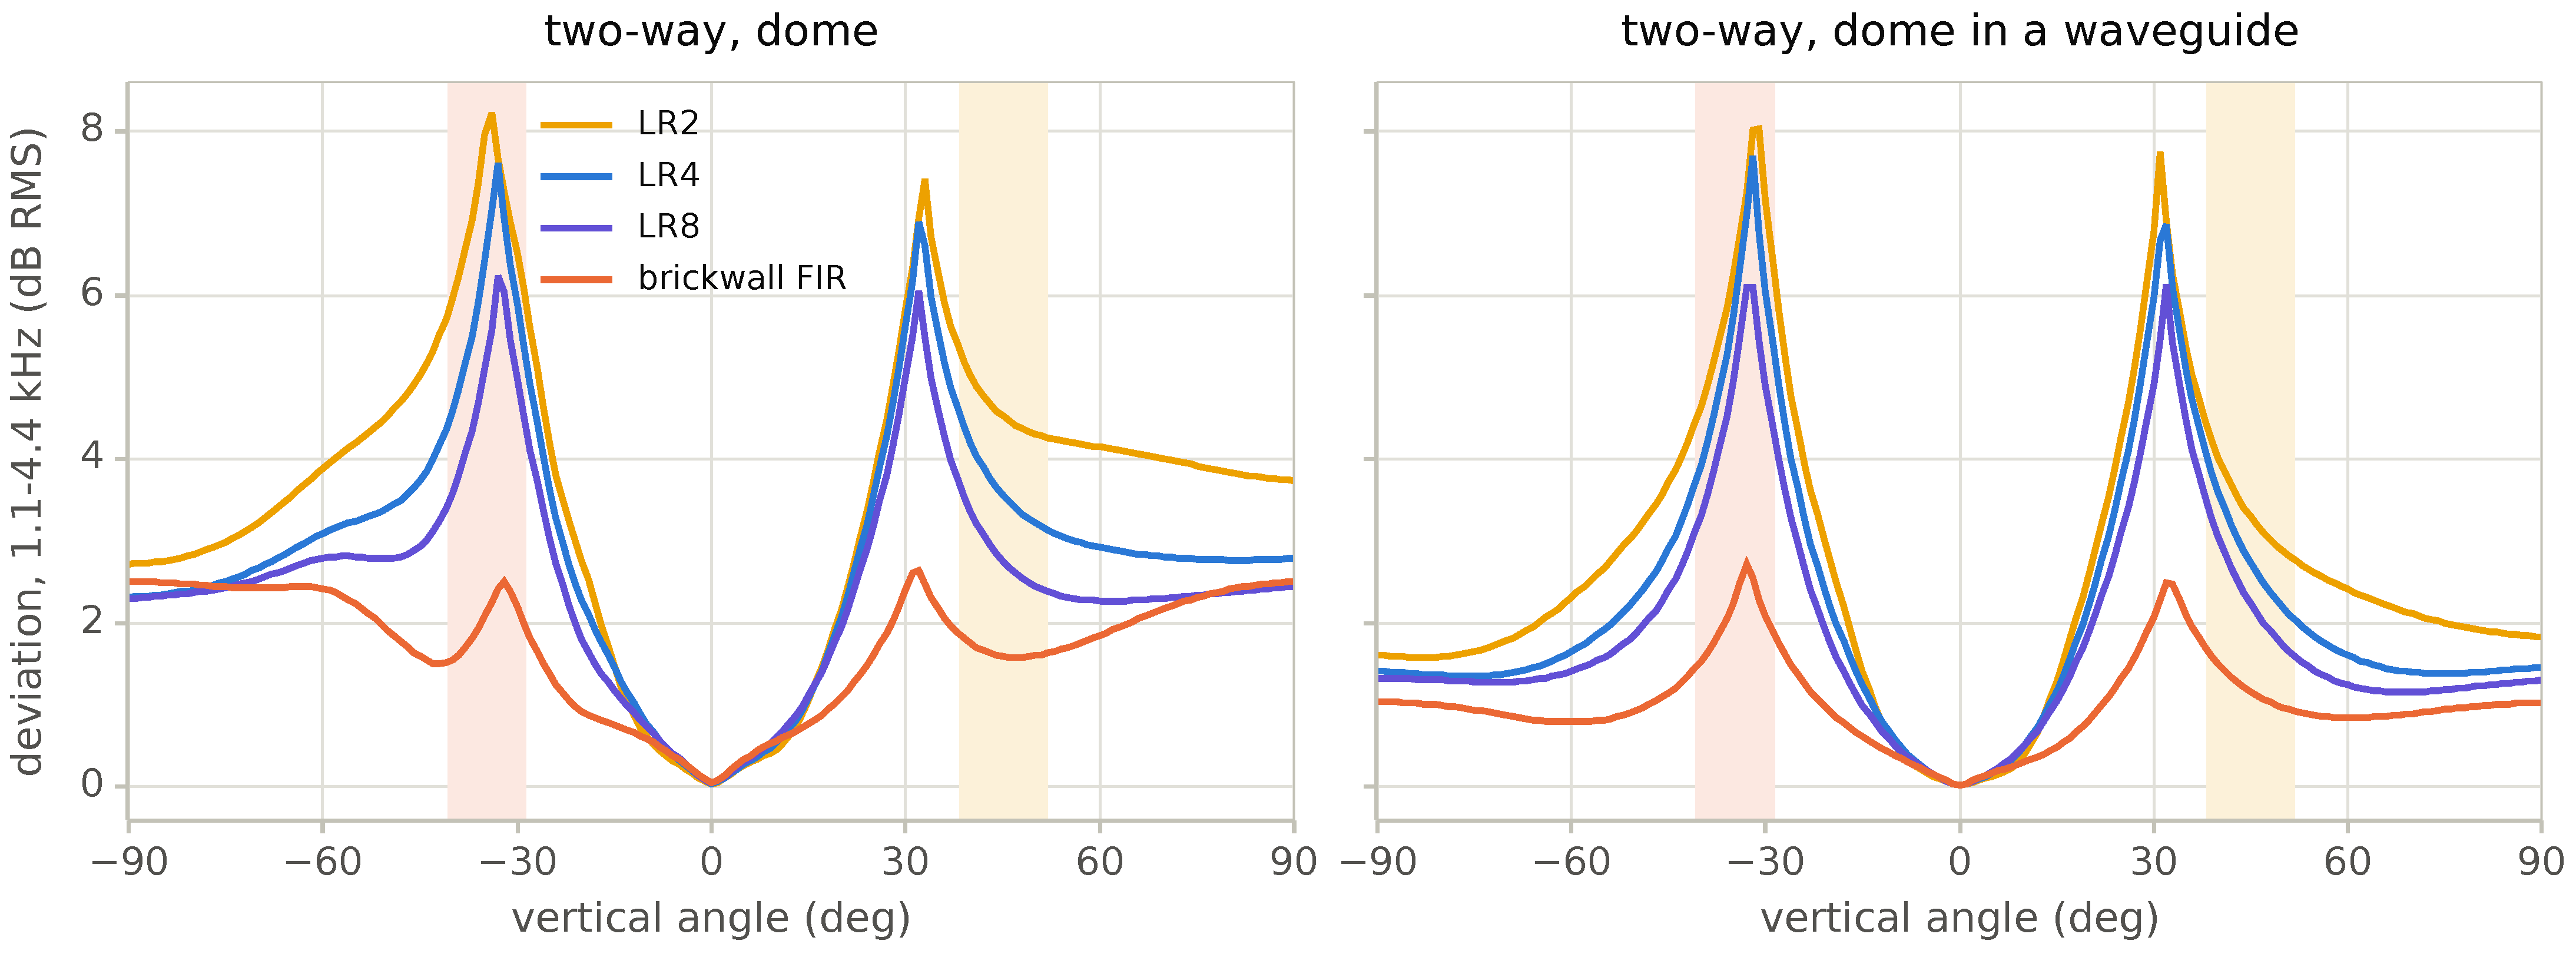
\includegraphics[width=\textwidth]{vertical_colouration}
\caption{Deviation of the response in each direction of the vertical orbit, within one octave of the
crossover, and the directions of the rooms' floor and ceiling bounces (shaded, 10--90\,\%).}
\label{fig:verticalcol}
\end{figure}

Along the vertical orbit (figure~\ref{fig:verticalcol}) the deviation peaks near the first null, at
$-33^\circ$ and $+32^\circ$ with the plain dome: 8.3 and 7.4\,dB RMS with LR2, 7.6 and 7.0 with LR4, 6.5
and 6.1 with LR8, 2.5 and 2.7 with the brickwall. The floor bounces of the 300 rooms sit on the lower
peak; the ceiling bounces on the upper one's shoulder.

\subsection{Results}

\begin{table}[t]
\centering
\caption{Averaged curves within one octave of the crossover (dB): RMS deviation from the straight line
of the PIR, of the PIR with the fitted weights, of the rooms' steady state and early sound (median of
the 300); deepest dip of the PIR and of the rooms' steady state.}
\label{tab:anomalies}
\small
\begin{tabular}{lrrrrrr}
\toprule
& \multicolumn{4}{c}{RMS deviation} & \multicolumn{2}{c}{deepest dip} \\
& PIR & fitted & rooms & rooms & PIR & rooms \\
& & & steady & early & & steady \\
\midrule
\rows{anomalies}
\bottomrule
\end{tabular}
\end{table}

\begin{table}[t]
\centering
\caption{Colouration of the paths, upright two-way: RMS deviation within one octave of the crossover
(dB), weighted by the PIR, by the fitted weights, and by the rooms (median of the 300): every path,
the first reflections, the floor and ceiling bounces; and the deepest dip of the floor and ceiling
bounces.}
\label{tab:colouration}
\small
\begin{tabular}{lrrrrrr}
\toprule
& PIR & fitted & rooms & rooms & rooms & floor, ceiling \\
& weights & weights & steady & reflections & floor, ceiling & deepest dip \\
\midrule
\rows{colouration}
\bottomrule
\end{tabular}
\end{table}

\begin{figure}[t]
\centering
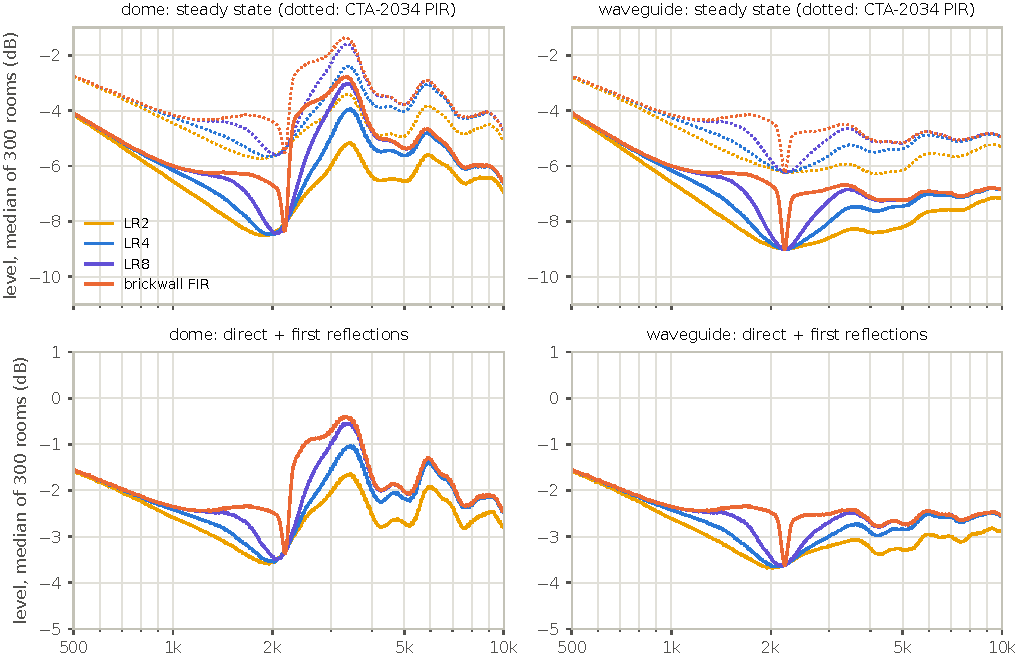
\includegraphics[width=\textwidth]{crossovers}
\caption{Median in-room response of the 300 rooms with the four crossovers, steady state (top, the PIR
dotted) and early sound (bottom); plain dome (left), dome in a waveguide (right).}
\label{fig:crossovers}
\end{figure}

\begin{figure}[t]
\centering
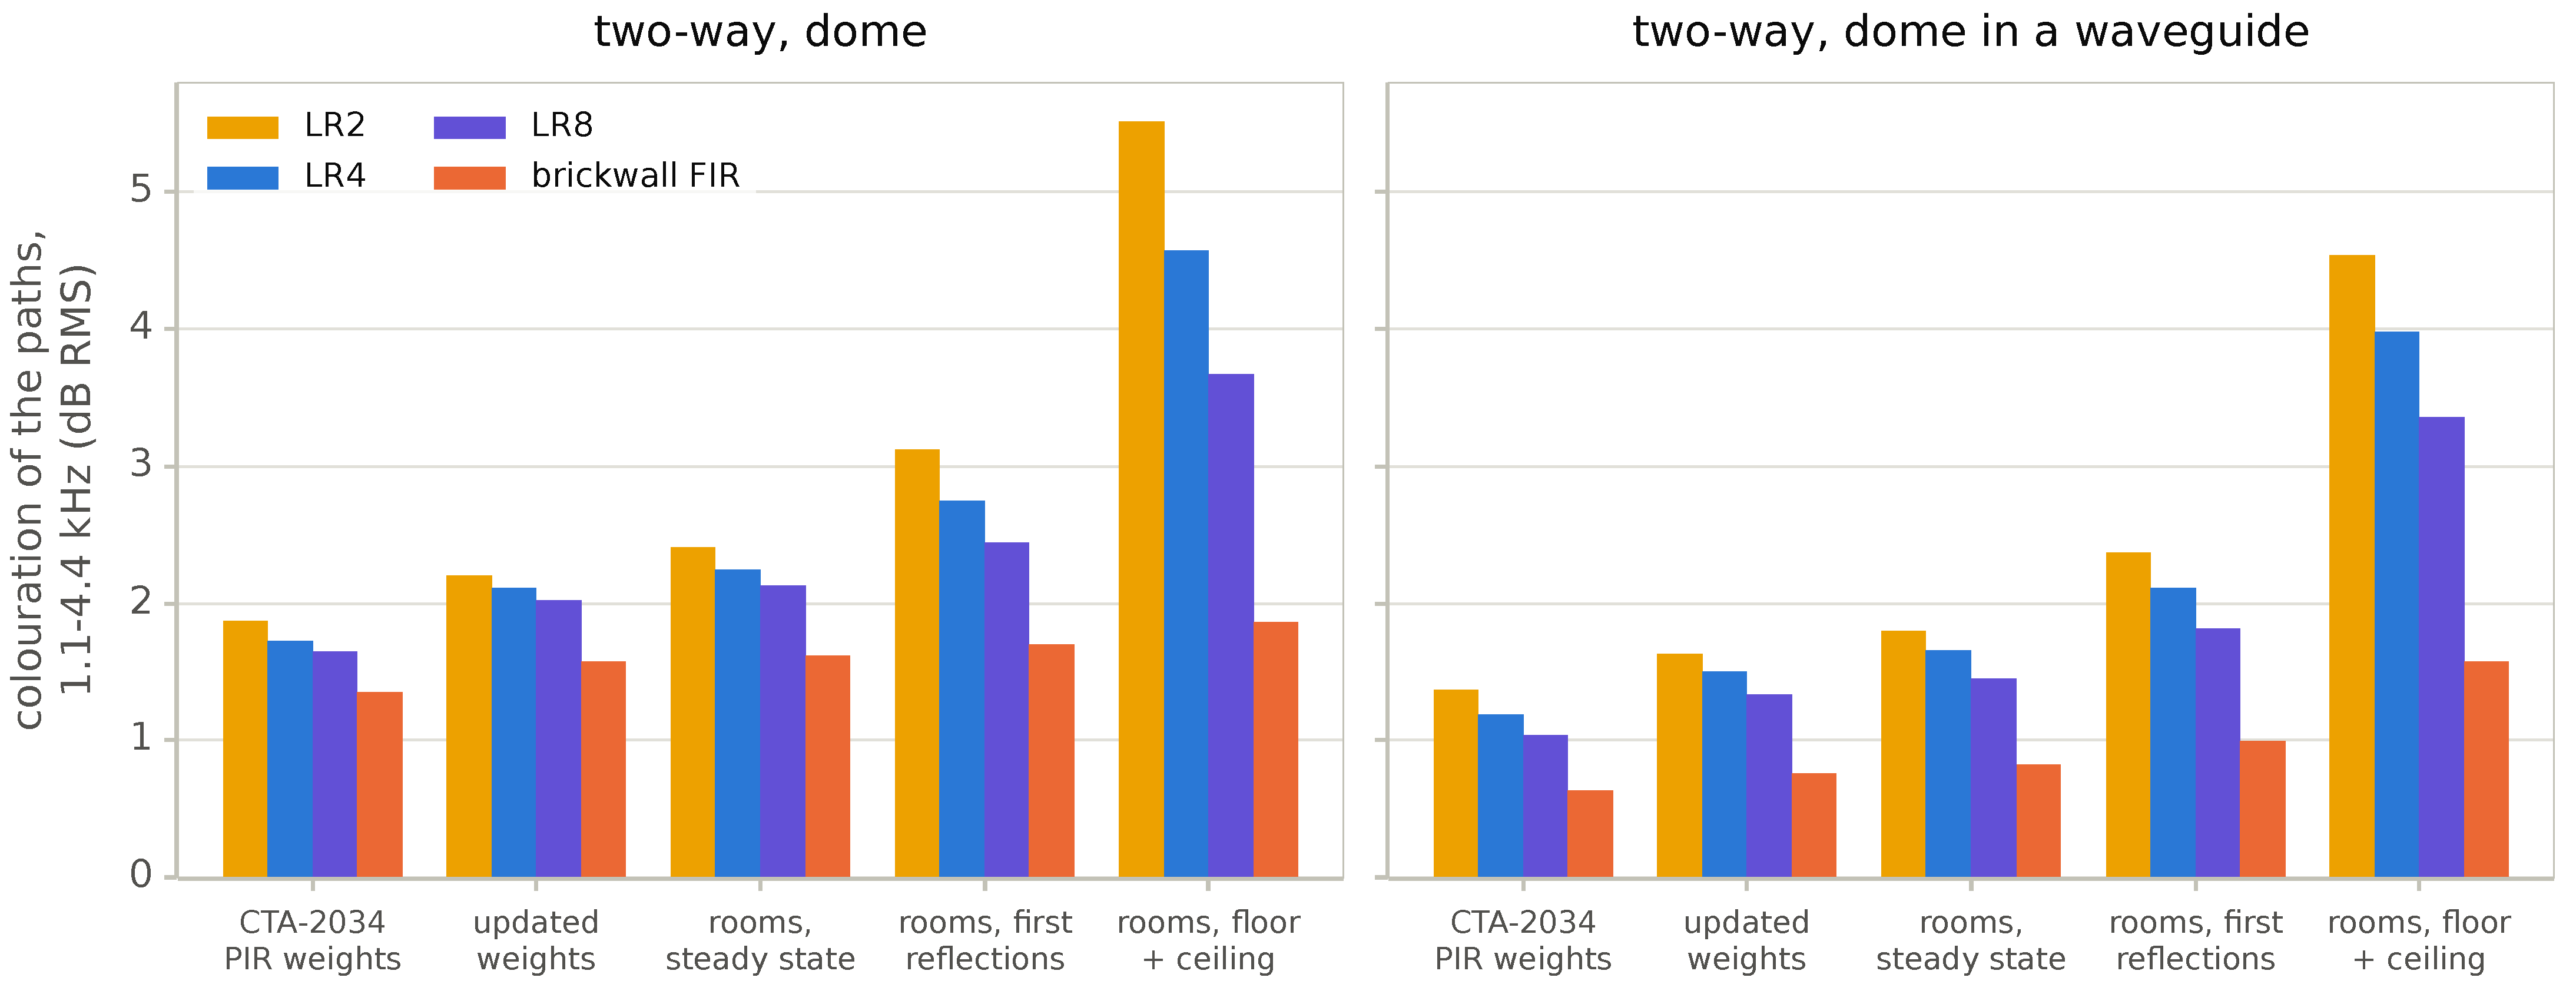
\includegraphics[width=\textwidth]{colouration}
\caption{Colouration of the paths with the four crossovers, upright two-way.}
\label{fig:colouration}
\end{figure}

\emph{The averages flatter the low-slope crossover} (table~\ref{tab:anomalies},
figure~\ref{fig:crossovers}). At the crossover frequency the four crossovers give the same response,
each driver at half amplitude and in phase; they differ by the width of the band where both drivers
play. In the rooms' averaged response the plain dome's LR2 deviates by \ncurveDomeLrTwoRoom\,dB RMS,
the LR4 by \ncurveDomeLrFourRoom, the brickwall by \ncurveDomeFirRoom; the deepest dips are
\ncurveDomeLrTwoRoomDip, \ncurveDomeLrFourRoomDip\ and \ncurveDomeFirRoomDip\,dB, the brickwall's being its
narrow notch at the crossover. With the plain dome the brickwall also turns the LR4's broad dip into a
step of about 3\,dB to the dome's wider radiation, and the averaged curve is no smoother. With the
waveguide there is no step: \ncurveWgLrFourRoom\ against \ncurveWgFirRoom\,dB (\ncurveWgLrTwoRoom\ with LR2).
The PIR ranks the crossovers the same way.

\emph{The paths rank them the other way} (table~\ref{tab:colouration}, figure~\ref{fig:colouration}).
The floor and ceiling bounces carry \ncolDomeLrTwoVert\,dB RMS with LR2, \ncolDomeLrFourVert\ with LR4 and
\ncolDomeFirVert\ with the brickwall (plain dome; \ncolWgLrTwoVert, \ncolWgLrFourVert\ and \ncolWgFirVert\
with the waveguide): from LR4 to the brickwall, \ncolDomeRedVert\ and \ncolWgRedVert\,\% less; LR2 is
\ncolDomeLrTwoMoreVert\,\% worse than LR4. For all the first reflections the brickwall removes
\ncolDomeRedRefl\ and \ncolWgRedRefl\,\%, for every path in steady state \ncolDomeRedSteady\ and
\ncolWgRedSteady\,\%. The deepest dip of the floor and ceiling bounces changes little
(\ncolDomeLrFourVertDip\ against \ncolDomeFirVertDip\,dB with the plain dome, \ncolWgLrFourVertDip\ against
\ncolWgFirVertDip\,dB with the waveguide): the brickwall's notches are as deep, ten to thirteen times
narrower, about a thirtieth of an octave against a third.

\emph{How much the averages hide.} With the plain dome and LR4, the floor and ceiling bounces carry
\ncolDomeLrFourVert\,dB RMS within an octave of the crossover and the rooms' averaged response shows
\ncurveDomeLrFourRoom\,dB: the averaging divides the colouration by about 3.4. With LR2 it divides it by 5
(\ncolDomeLrTwoVert\ against \ncurveDomeLrTwoRoom\,dB), with the brickwall by 1.4. The lower the slope, the
wider the band where the drivers interfere, the more directions see the notch at different frequencies,
and the more the average fills it.

\emph{The standard's weights} give the paths' colouration less weight than the rooms do
(\ncolDomeLrFourPir\ against \ncolDomeLrFourSteady\,dB with the plain dome and LR4), because the PIR leans
on the Listening Window, where vertical lobing does not show; they show a slightly smaller gain from
the brickwall (\ncolDomeRedPir\ against \ncolDomeRedSteady\,\% with the plain dome, \ncolWgRedPir\ against
\ncolWgRedSteady\,\% with the waveguide). The updated weights sit in between.

\clearpage
\subsection{Interference at the ears}
\label{sec:interference}

Every response so far adds the paths in power, as if each were heard on its own. At a fixed point the
direct sound and the reflections add as pressures: a reflection delayed by $\tau$ digs a notch every
$1/\tau$ into the response, a comb. To see what the comb does to the comparison, the direct sound and
the images up to the third order were added with their phases at fourteen points: the two ears,
17.5\,cm apart and without a head, of seven head positions (the reference one, 10\,cm to either side,
10\,cm forward and back, 5\,cm up and down). Each image keeps the square root of its energy weight as a
real, positive reflection factor, and the loudspeaker's response in the direction its path leaves in;
the diffuse field is still added in energy. The ear does not resolve the fine comb of a late
reflection, so every response is smoothed by the auditory filters of Glasberg and Moore
\cite{glasberg1990}, rounded exponentials one ERB wide (\nerbCrossover\,Hz at the crossover, about a sixth
of an octave), computed on a 4\,Hz grid, before its deviation within one octave of the crossover is
taken. The images' energy matches the study's within $\ncohCheck$\,dB. An omnidirectional source in the
same rooms shows the combs the rooms produce on their own.

\begin{table}[t]
\centering
\caption{Deviation within one octave of the crossover (dB RMS, median of the 300 rooms) of the paths
added in power at the reference point, and with their phases: at one point (median of the fourteen),
at the two ears averaged in power, at the fourteen points averaged. Upright two-way; responses
smoothed by the auditory filters.}
\label{tab:coherent}
\small
\begin{tabular}{lrrrrrrrr}
\toprule
& \multicolumn{4}{c}{steady state} & \multicolumn{4}{c}{early sound} \\
\cmidrule(lr){2-5}\cmidrule(lr){6-9}
& power & point & ears & 14 pts & power & point & ears & 14 pts \\
\midrule
\rows{coherent}
\bottomrule
\end{tabular}
\end{table}

\begin{figure}[t]
\centering
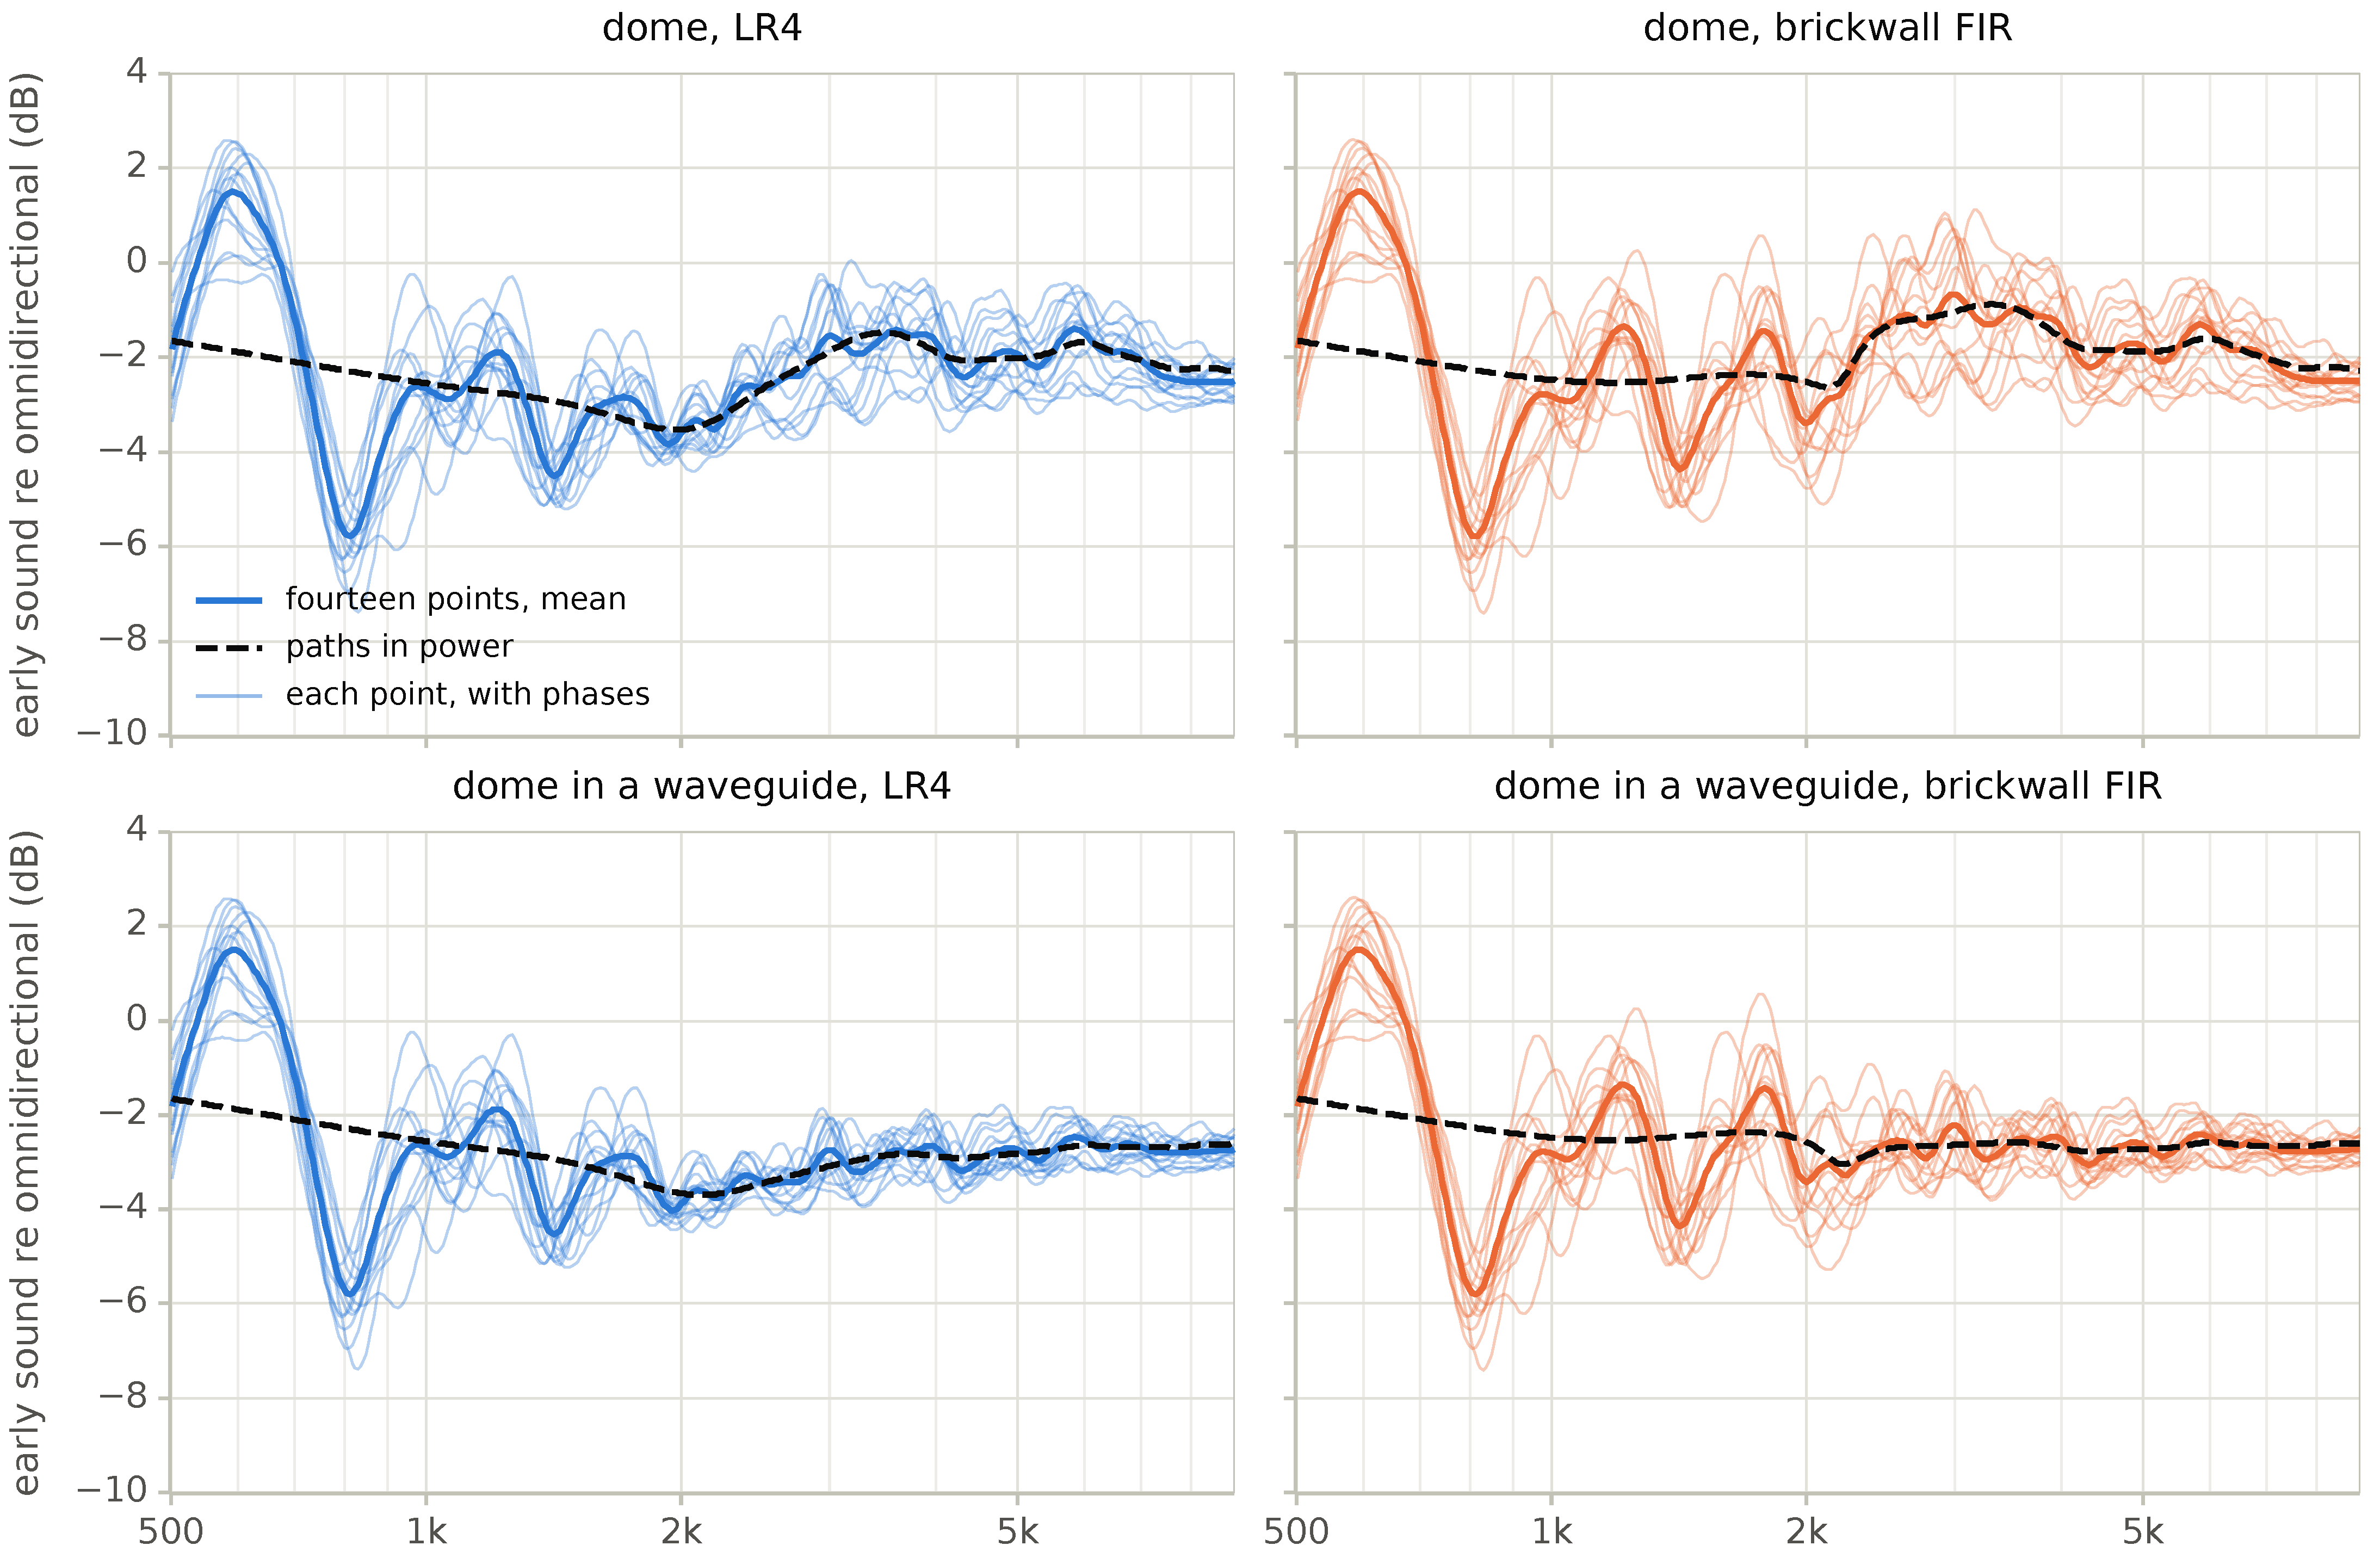
\includegraphics[width=\textwidth]{interference}
\caption{Early sound in the living room of figure~\ref{fig:setup}, relative to an omnidirectional
source: the paths added in power at the reference point (dashed), and with their phases at each of
the fourteen points (thin) and averaged over them (thick); smoothed by the auditory filters.}
\label{fig:interference}
\end{figure}

\begin{figure}[t]
\centering
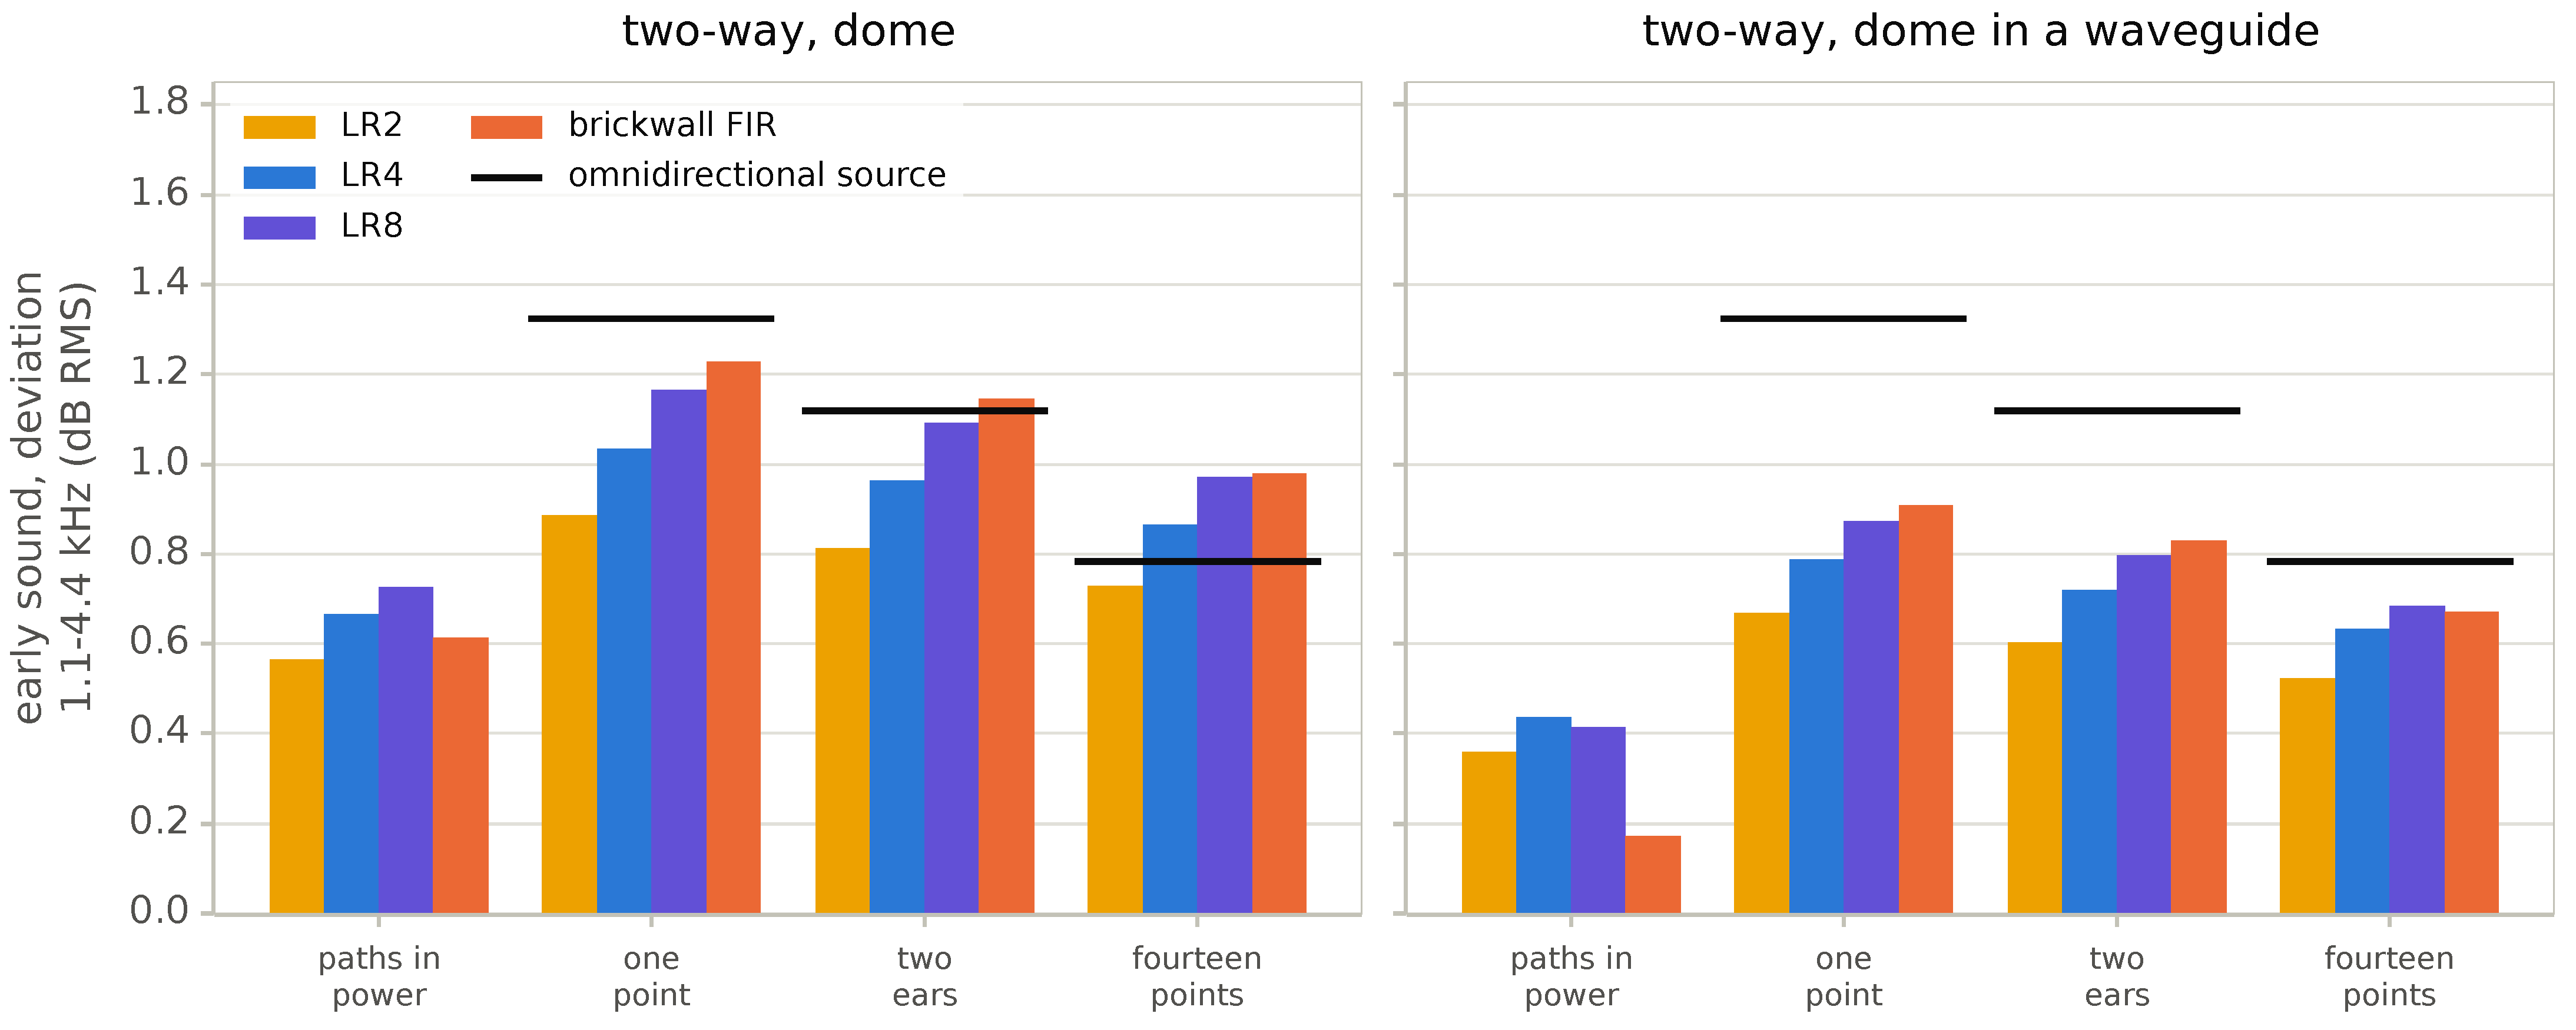
\includegraphics[width=\textwidth]{interference_summary}
\caption{Deviation of the early sound within one octave of the crossover (median of the 300 rooms):
the paths added in power, then with their phases at one point, at the two ears averaged, at the
fourteen points averaged. Black lines: an omnidirectional source, the combs of the rooms alone.}
\label{fig:interference-summary}
\end{figure}

\emph{In steady state the phases change little} (table~\ref{tab:coherent}). The diffuse field, added in
energy, fills the combs: at one point the deviation grows by \ncohSteadyGainMin\ to \ncohSteadyGainMax\,dB,
and the crossovers keep their order (plain dome: LR2 \ncohDomeLrTwoSteadyPoint, LR4
\ncohDomeLrFourSteadyPoint, brickwall \ncohDomeFirSteadyPoint\,dB; waveguide: \ncohWgLrFourSteadyPoint\ with LR4
against \ncohWgFirSteadyPoint\ with the brickwall). The omnidirectional source's combs leave
\ncohOmniSteadyPoint\,dB.

\emph{The early sound at one point is another matter} (figures~\ref{fig:interference}
and~\ref{fig:interference-summary}). There the direct sound meets the floor and ceiling bounces,
\ndelayFloor\ and \ndelayCeiling\,ms later in the median room: their combs, a few hundred hertz apart, are
about as wide as the auditory filters and survive the smoothing. The omnidirectional source shows
\ncohOmniEarlyPoint\,dB RMS within an octave of the crossover at one point, more than any crossover in
power (\ncohDomeLrEightEarlyEnergy\,dB at most, LR8 with the plain dome). The loudspeakers fall in between,
from \ncohDomeLrTwoEarlyPoint\ (LR2) to \ncohDomeFirEarlyPoint\,dB (brickwall) with the plain dome, from
\ncohWgLrTwoEarlyPoint\ to \ncohWgFirEarlyPoint\,dB with the waveguide, and the brickwall comes last: the
smoothest in power with the waveguide (\ncohWgFirEarlyEnergy\ against \ncohWgLrFourEarlyEnergy\,dB for LR4),
it is the roughest at one point. The Linkwitz-Riley notch takes the floor and ceiling bounces out
around the crossover, and their comb with them: in the living room the fourteen points close in on
the energy sum around 2\,kHz with LR4, not with the brickwall, which leaves the reflections and their
comb intact. Averaging the two ears or the fourteen points narrows the gaps without closing them
(\ncohWgLrFourEarlySpatial\ against \ncohWgFirEarlySpatial\,dB over the fourteen points with the waveguide).

What the comb measures is the room, not the crossover: a source without a crossover shows it
everywhere, and a crossover that notches the reflections near its frequency removes it there, with
part of the reflections' energy. Whether that sounds better is for listening tests to tell. A single
reflection's comb colours the sound less for two ears than for one (binaural decoloration
\cite{salomons1995}), and the reflections' own spectrum, which the colouration of the paths measures,
is what the ear ascribes to the room. Interference thus leaves the steady-state picture as it is; at a
fixed point it trades the crossover's colouration of the reflections for the comb those reflections
cause.

% =============================================================================================
\section{Discussion}

\subsection{The three objections}

\emph{The vertical weight.} In these rooms the floor and ceiling bring as large a share of the first
reflections' energy as the Early Reflections give them, and their bounces leave where the standard
looks. They do arrive first, and where the side walls are treated they bring half of it, a little
more than the standard's 40\,\%. The objection holds for the sound power: the two orbits weigh the
plane without interference as much as the one with it, and miss half of the power lost to lobing. That
bias is the same for horizontal and vertical lobing; for an upright loudspeaker it falls on the
vertical one.

\emph{The Listening Window.} Its narrow vertical extent is not what hides the lobing: the direct sound
of a seated listener does not see vertical lobing either, and laying the loudspeaker on its side shows
what the window guards against. What hides it is the averaging every curve shares, the room's own
average included. The floor and ceiling bounces of an LR4 two-way carry notches of 10 to 40\,dB, a third
of an octave wide, which fall at different frequencies in different directions; the averages turn them
into a dip of 2\,dB. The lower the slope, the more the averages flatter the crossover: the in-room curve
and the PIR rank LR2 as the smoothest of the Linkwitz-Riley crossovers, while its reflections are the
most coloured. In that form, the objection holds.

\emph{The brickwall crossover.} It reduces the colouration of the floor and ceiling bounces by about
60\,\%, with or without the waveguide, and of all the first reflections by 38 to 53\,\%. Its notches are as
deep as the Linkwitz-Riley ones, ten to thirteen times narrower. Whether the in-room curve becomes smoother depends
on the drivers: where the woofer beams at the crossover and the tweeter does not, the brickwall turns
the lobing dip into a step of directivity. Matching the directivities at the crossover (a waveguide)
and narrowing the band where both drivers play (a steep crossover) address two different causes of the
off-axis colouration.

\subsection{An updated weighting}

What the rooms ask for is simple to state:
\begin{itemize}
\item the sound power over the sphere, which near-field scanners and spherical measurements now give,
instead of two orbits;
\item for the steady-state in-room response, about $0.1\,\mathrm{LW} + 0.9\,\mathrm{SP}$: the room
behaves mostly as a sound-power meter, the direct sound adding a little forward weight;
\item for the early sound, which carries the reflections heard with the direct sound, about
$0.4\,\mathrm{LW} + 0.5\,\mathrm{ER} + 0.1\,\mathrm{SP}$.
\end{itemize}
Fitted to the received energy, the first set of weights predicts the rooms within their own spread. It
does not undo the averaging, though: no weighted mean of power responses shows the notch a single
reflection carries. That has to be read direction by direction, on the polar maps or with a measure
like the colouration of the paths used here, in the directions where the floor and ceiling bounces
leave, $-30$ to $-40^\circ$ and $+40$ to $+50^\circ$ at usual listening distances.

\subsection{Limits}

The rooms are shoeboxes, with uniform absorption per surface except for the patches, textbook
coefficients and a hybrid specular-diffuse model; real rooms have furniture in the paths, openings,
irregular shapes. Their reverberation and their energy shares follow from the room constant and are
not specific to this model, but the share of each first reflection depends on the materials at the
reflection point. Paths are added in energy, except in section~\ref{sec:interference}, where the
images meet with their phases at points without a head; the room's modes below about 200\,Hz are
outside the study. The early sound is an energy sum too; hearing weighs
reflections differently from their energy (binaural decoloration of lateral reflections, the
salience of the floor bounce in the median plane \cite{bech1996,olive1989}), which no weighting of
power responses captures. The colouration metrics are physical measures: a narrow notch is harder to
hear than a broad one of the same depth \cite{bucklein1981}, and the RMS deviation accounts for that only
through its width. The loudspeaker is one two-way bookshelf in two versions; a three-way, a cardioid, a
floor-standing loudspeaker or a larger listening distance would change the numbers, not the method.
Finally the study uses CTA-2034-A; its revision B was not checked.

% =============================================================================================
\section{Conclusion}

Seen as weights over the directions of the sphere, CTA-2034's curves and a room can be compared
directly. In 300 simulated domestic rooms the standard looks for the first reflections in the right
directions and gives the floor and ceiling the right share of them; its Listening Window matches where
listeners sit. Its weights do not match the energy received: the first reflections carry
\nfirstShare\,\% of the steady-state energy, not 44\,\%, and the rooms are predicted to within their own
spread by about $0.1\,\mathrm{LW} + 0.9\,\mathrm{SP}$ with the sound power of the whole sphere, which
two orbits underestimate where drivers interfere. Any average, the room's included, fills the notches
the crossover digs into each reflection, and flatters the low-slope crossovers most. Read path by path,
a brickwall crossover removes about 60\,\% of the colouration of the floor and ceiling bounces; it gives a
smoother in-room response only when the drivers' directivities match at the crossover. Added with their
phases at the ears, the paths leave the steady state as it is; at a fixed point the early sound
carries the comb of the floor and ceiling bounces, which a Linkwitz-Riley notch removes near the
crossover along with the reflections, and which hearing with two ears attenuates.

% =============================================================================================
\begin{thebibliography}{99}

\bibitem{cta2034a} ANSI/CTA-2034-A, \emph{Standard Method of Measurement for In-Home Loudspeakers},
Consumer Technology Association, 2015 (R2020).

\bibitem{cta2034b} ANSI/CTA-2034-B, \emph{Standard Method of Measurement for In-Home Loudspeakers},
Consumer Technology Association, July 2024.

\bibitem{devantier2002} A. Devantier, ``Characterizing the Amplitude Response of Loudspeaker Systems,''
113th AES Convention, preprint 5638, 2002.

\bibitem{toole2018} F. E. Toole, \emph{Sound Reproduction: The Acoustics and Psychoacoustics of
Loudspeakers and Rooms}, 3rd ed., Routledge, 2018.

\bibitem{olive2004} S. E. Olive, ``A Multiple Regression Model for Predicting Loudspeaker Preference
Using Objective Measurements: Part II -- Development of the Model,'' 117th AES Convention, preprint
6190, 2004.

\bibitem{demion2026} A. Demion, ``Brickwall FIR Crossovers Against LR24 on Four-Way Studio Monitors,''
DEM Audio blog, October 2026, \url{https://demaudio.com/blog/brickwall-fir-vs-lr24/}.

\bibitem{turntable2026} ``Polar Measurements on a Small Turntable: How Well Can the Rotation Center Be
Corrected?'', technical report, 2026, \url{https://github.com/Arnwald/turntable-rotation-center-study}.

\bibitem{urban2004} M. Urban, C. Heil, C. Pignon, C. Combet, P. Bauman, ``The Distributed Edge Dipole
(DED) Model for Cabinet Diffraction Effects,'' \emph{J. Audio Eng. Soc.}, vol.~52, no.~10, 2004.

\bibitem{allen1979} J. B. Allen, D. A. Berkley, ``Image Method for Efficiently Simulating Small-Room
Acoustics,'' \emph{J. Acoust. Soc. Am.}, vol.~65, no.~4, pp.~943--950, 1979.

\bibitem{kuttruff2016} H. Kuttruff, \emph{Room Acoustics}, 6th ed., CRC Press, 2016.

\bibitem{hopkins1948} H. F. Hopkins, N. R. Stryker, ``A Proposed Loudness-Efficiency Rating for
Loudspeakers and the Determination of System Power Requirements for Enclosures,'' \emph{Proc. IRE},
vol.~36, no.~3, pp.~315--335, 1948.

\bibitem{iso9613} ISO 9613-1, \emph{Acoustics -- Attenuation of sound during propagation outdoors --
Part 1: Calculation of the absorption of sound by the atmosphere}, 1993.

\bibitem{diaz2005} C. D\'iaz, A. Pedrero, ``The reverberation time of furnished rooms in dwellings,''
\emph{Applied Acoustics}, vol.~66, no.~8, 2005.

\bibitem{bech1996} S. Bech, ``Timbral aspects of reproduced sound in small rooms. II,'' \emph{J. Acoust.
Soc. Am.}, vol.~99, no.~6, 1996.

\bibitem{olive1989} S. E. Olive, F. E. Toole, ``The Detection of Reflections in Typical Rooms,''
\emph{J. Audio Eng. Soc.}, vol.~37, no.~7/8, 1989.

\bibitem{bucklein1981} R. B\"ucklein, ``The Audibility of Frequency Response Irregularities,'' \emph{J. Audio
Eng. Soc.}, vol.~29, no.~3, pp.~126--131, 1981.

\bibitem{glasberg1990} B. R. Glasberg, B. C. J. Moore, ``Derivation of auditory filter shapes from
notched-noise data,'' \emph{Hearing Research}, vol.~47, pp.~103--138, 1990.

\bibitem{salomons1995} A. M. Salomons, \emph{Coloration and Binaural Decoloration of Sound due to
Reflections}, PhD thesis, Delft University of Technology, 1995.

\end{thebibliography}

\end{document}
